\documentclass[aps,prb,reprint,noshowkeys,linenumbers,superscriptaddress]{revtex4-1}
\usepackage{subcaption}
\usepackage{bm,graphicx,tabularx,array,booktabs,dcolumn,xcolor,microtype,multirow,amscd,amsmath,amssymb,amsfonts,physics,siunitx,mhchem}
\usepackage[utf8]{inputenc}
\usepackage[T1]{fontenc}
\usepackage{txfonts}

\usepackage[normalem]{ulem}
\definecolor{hughgreen}{RGB}{0, 128, 0}
\newcommand{\titou}[1]{\textcolor{red}{#1}}
\newcommand{\hugh}[1]{\textcolor{hughgreen}{#1}}
\newcommand{\trash}[1]{\textcolor{red}{\sout{#1}}}
\newcommand{\trashHB}[1]{\textcolor{orange}{\sout{#1}}}

\usepackage[
	colorlinks=true,
    citecolor=blue,
    linkcolor=blue,
    filecolor=blue,      
    urlcolor=blue,	
    breaklinks=true
	]{hyperref}
\urlstyle{same}

\newcommand{\ctab}{\multicolumn{1}{c}{---}}
\newcommand{\latin}[1]{#1}
%\newcommand{\latin}[1]{\textit{#1}}
\newcommand{\ie}{\latin{i.e.}}
\newcommand{\eg}{\latin{e.g.}}
\newcommand{\mc}{\multicolumn}
\newcommand{\fnm}{\footnotemark}
\newcommand{\fnt}{\footnotetext}
\newcommand{\mcc}[1]{\multicolumn{1}{c}{#1}}
\newcommand{\mr}{\multirow}

% operators
\newcommand{\bH}{\mathbf{H}}
\newcommand{\bV}{\mathbf{V}}
\newcommand{\bh}{\mathbf{h}}
\newcommand{\bQ}{\mathbf{Q}}
\newcommand{\bSig}{\mathbf{\Sigma}}
\newcommand{\br}{\mathbf{r}}
\newcommand{\bp}{\mathbf{p}}
\newcommand{\cP}{\mathcal{P}}
\newcommand{\cS}{\mathcal{S}}
\newcommand{\cT}{\mathcal{T}}
\newcommand{\cC}{\mathcal{C}}
\newcommand{\PT}{\mathcal{PT}}

\newcommand{\EPT}{E_{\PT}}
\newcommand{\laPT}{\lambda_{\PT}}

\newcommand{\EEP}{E_\text{EP}}
\newcommand{\laEP}{\lambda_\text{EP}}


\newcommand{\Ne}{N} % Number of electrons
\newcommand{\Nn}{M} % Number of nuclei
\newcommand{\hI}{\Hat{I}}
\newcommand{\hH}{\Hat{H}}
\newcommand{\hS}{\Hat{S}}
\newcommand{\hT}{\Hat{T}}
\newcommand{\hW}{\Hat{W}}
\newcommand{\hV}{\Hat{V}}
\newcommand{\hc}[2]{\Hat{c}_{#1}^{#2}}
\newcommand{\hn}[1]{\Hat{n}_{#1}}
\newcommand{\n}[1]{n_{#1}}
\newcommand{\Dv}{\Delta v}

\newcommand{\ra}{\rightarrow}
\newcommand{\up}{\uparrow}
\newcommand{\dw}{\downarrow}

\newcommand{\updot}{%
  \mathrel{\ooalign{\hfil$\vcenter{
    \hbox{$\scriptscriptstyle\bullet$}}$\hfil\cr$\uparrow$\cr}
  }%
}
\newcommand{\dwdot}{%
  \mathrel{\ooalign{\hfil$\vcenter{
    \hbox{$\scriptscriptstyle\bullet$}}$\hfil\cr$\downarrow$\cr}
  }%
}
\newcommand{\vac}{%
  \mathrel{\ooalign{\hfil$\vcenter{
    \hbox{$\scriptscriptstyle\bullet$}}$\hfil\cr$ $\cr}
  }%
}

\newcommand{\uddot}{%
  \mathrel{\ooalign{\hfil$\vcenter{
    \hbox{$\scriptscriptstyle\bullet$}}$\hfil\cr$\uparrow\downarrow$\cr}
  }%
}

% Center tabularx columns
\newcolumntype{Y}{>{\centering\arraybackslash}X}

% HF rotation angles
\newcommand{\ta}{\theta_{\alpha}}
\newcommand{\tb}{\theta_{\beta}}

% Some constants
\renewcommand{\i}{\mathrm{i}} % Imaginary unit
\newcommand{\e}{\mathrm{e}} % Euler number
\newcommand{\rc}{r_{\text{c}}}
\newcommand{\lc}{\lambda_{\text{c}}}
\newcommand{\lep}{\lambda_{\text{EP}}}

% Blackboard bold
\newcommand{\bbR}{\mathbb{R}}
\newcommand{\bbC}{\mathbb{C}}

\newcommand{\Lup}{\mathcal{L}^{\uparrow}}
\newcommand{\Ldown}{\mathcal{L}^{\downarrow}}
\newcommand{\Lsi}{\mathcal{L}^{\sigma}}
\newcommand{\Rup}{\mathcal{R}^{\uparrow}}
\newcommand{\Rdown}{\mathcal{R}^{\downarrow}}
\newcommand{\Rsi}{\mathcal{R}^{\sigma}}


\newcommand{\LCPQ}{Laboratoire de Chimie et Physique Quantiques (UMR 5626), Universit\'e de Toulouse, CNRS, UPS, France.}
\newcommand{\UCAM}{Department of Chemistry, University of Cambridge, Lensfield Road, Cambridge, CB2 1EW, U.K.}
\newcommand{\UOX}{Physical and Theoretical Chemical Laboratory, Department of Chemistry, University of Oxford, Oxford, OX1 3QZ, U.K.}
\begin{document}	

\title{Perturbation theory in the complex plane: Exceptional points and where to find them}

\author{Antoine \surname{Marie}}
\affiliation{\LCPQ}
\author{Hugh G.~A.~\surname{Burton}}
\email{hugh.burton@chem.ox.ac.uk}
\affiliation{\UOX}
\author{Pierre-Fran\c{c}ois \surname{Loos}}
\email{loos@irsamc.ups-tlse.fr}
\affiliation{\LCPQ}


\begin{abstract}
In this review, we explore the extension of quantum chemistry in the complex plane.
We observe that the physics of a quantum system is intimately connected to the position of the energy singularities in the complex plane. 
After a presentation of the fundamental notions of quantum chemistry and perturbation theory in the complex plane, we provide a historical overview of the various research activities that have been performed on the physic of singularities.
\end{abstract}

\maketitle

%%%%%%%%%%%%%%%%%%%%%%%
\section{Introduction}
\label{sec:intro}
%%%%%%%%%%%%%%%%%%%%%%%

%======================%
\subsection{Background}
%=======================%

Due to the ubiquitous influence of processes involving electronic excited states in physics, chemistry, and biology, their faithful description from first principles has been one of the grand challenges faced by theoretical chemists since the dawn of computational chemistry. 
Accurately predicting ground- and excited-state energies (hence excitation energies) is particularly valuable in this context, and it has concentrated most of the efforts within the community.
An armada of theoretical and computational methods have been developed to this end, each of them being plagued by its own flaws. 
The fact that none of these methods is successful in every chemical scenario has encouraged chemists to carry on the development of new excited-state methodologies, their main goal being to get the most accurate excitation energies (and properties) at the lowest possible computational cost in the most general context.

One common feature of all these methods is that they rely on the notion of quantised energy levels of Hermitian quantum mechanics, in which the different electronic states of a molecule or an atom are energetically ordered, the lowest being the ground state while the higher ones are excited states. 
Within this quantised paradigm, electronic states look completely disconnected from one another.
Many current methods study excited states using only ground-state information, creating a ground-state bias that leads to incorrect excitation energies.
However, one can gain a different perspective on quantisation extending quantum chemistry into the complex domain.
In a non-Hermitian complex picture, the energy levels are \textit{sheets} of a more complicated topological manifold called \textit{Riemann surface}, and they are smooth and continuous \textit{analytic continuation} of one another. 
In other words, our view of the quantised nature of conventional Hermitian quantum mechanics arises only from our limited perception of the more complex and profound structure of its non-Hermitian variant. \cite{MoiseyevBook,BenderPTBook}
The realisation that ground and excited states both emerge from one single mathematical structure with equal importance suggests that excited-state energies can be computed from first principles in their own right. 
One could then exploit the structure of these Riemann surfaces to develop methods that directly target excited-state energies without needing ground-state information. \cite{Burton_2019,Burton_2019a}

By analytically continuing the electronic energy $E(\lambda)$ in the complex domain (where $\lambda$ is a coupling parameter), the ground and excited states of a molecule can be smoothly connected.
This connection is possible because by extending real numbers to the complex domain, the ordering property of real numbers is lost.
Hence, electronic states can be interchanged away from the real axis since the concept of ground and excited states has been lost.
Amazingly, this smooth and continuous transition from one state to another has recently been experimentally realized in physical settings such as electronics, microwaves, mechanics, acoustics, atomic systems and optics. \cite{Bittner_2012,Chong_2011,Chtchelkatchev_2012,Doppler_2016,Guo_2009,Hang_2013,Liertzer_2012,Longhi_2010,Peng_2014, Peng_2014a,Regensburger_2012,Ruter_2010,Schindler_2011,Szameit_2011,Zhao_2010,Zheng_2013,Choi_2018,El-Ganainy_2018}

Exceptional points (EPs) are branch point singularities where two (or more) states become exactly degenerate. \cite{MoiseyevBook,Heiss_1988,Heiss_1990,Heiss_1999,Berry_2011,Heiss_2012,Heiss_2016,Benda_2018}
They are the non-Hermitian analogs of conical intersections, \cite{Yarkony_1996} which are ubiquitous in non-adiabatic processes and play a key role in photo-chemical mechanisms.
In the case of auto-ionising resonances, EPs have a role in deactivation processes similar to conical intersections in the decay of bound excited states. \cite{Benda_2018}
Although Hermitian and non-Hermitian Hamiltonians are closely related, the behaviour of their eigenvalues near degeneracies is starkly different.
For example, encircling non-Hermitian degeneracies at EPs leads to an interconversion of states, and two loops around the EP are necessary to recover the initial energy. \cite{MoiseyevBook,Heiss_2016,Benda_2018}
Additionally, the wave function picks up a geometric phase (also known as Berry phase \cite{Berry_1984}) and four loops are required to recover the initial wave function.
In contrast, encircling Hermitian degeneracies at conical intersections only introduces a geometric phase while leaving the states unchanged.
More dramatically, whilst eigenvectors remain orthogonal at conical intersections, at non-Hermitian EPs the eigenvectors themselves become equivalent, resulting in a \textit{self-orthogonal} state. \cite{MoiseyevBook}
More importantly here, although EPs usually lie off the real axis, these singular points are intimately related to the convergence properties of perturbative methods and avoided crossing on the real axis are indicative of singularities in the complex plane. \cite{BenderBook,Olsen_1996,Olsen_2000,Olsen_2019,Mihalka_2017a,Mihalka_2017b,Mihalka_2019}

%===================================%
\subsection{Illustrative Example}
\label{sec:example}
%===================================%

%%% FIG 1 %%%
\begin{figure*}[t]
	\begin{subfigure}{0.49\textwidth}
	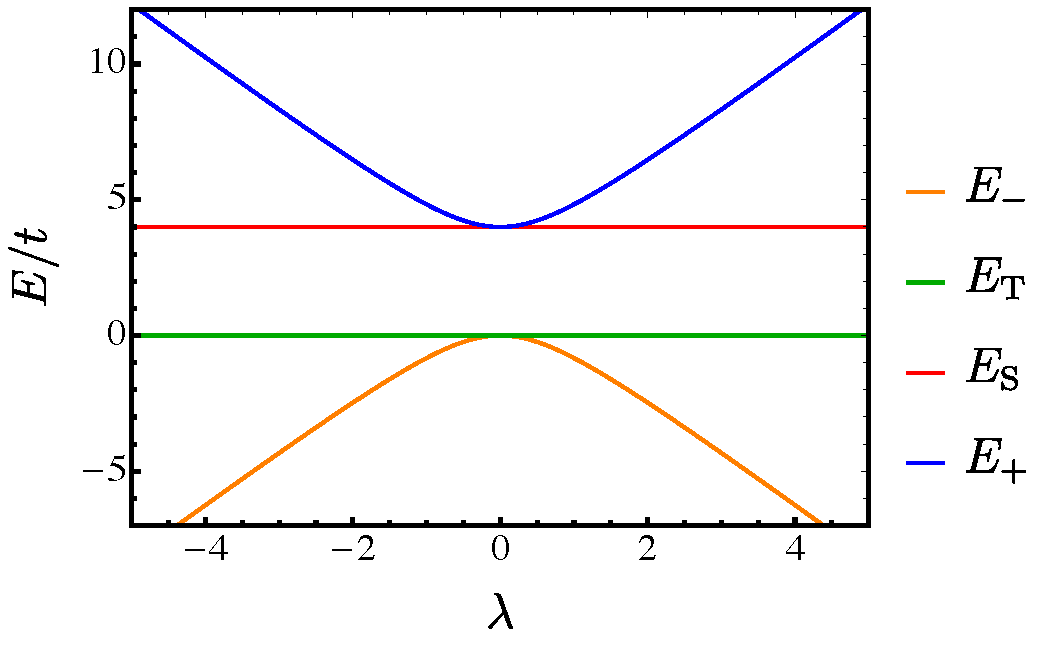
\includegraphics[height=0.65\textwidth]{fig1a}
	\subcaption{\label{subfig:FCI_real}}
    \end{subfigure}
	\begin{subfigure}{0.49\textwidth}
	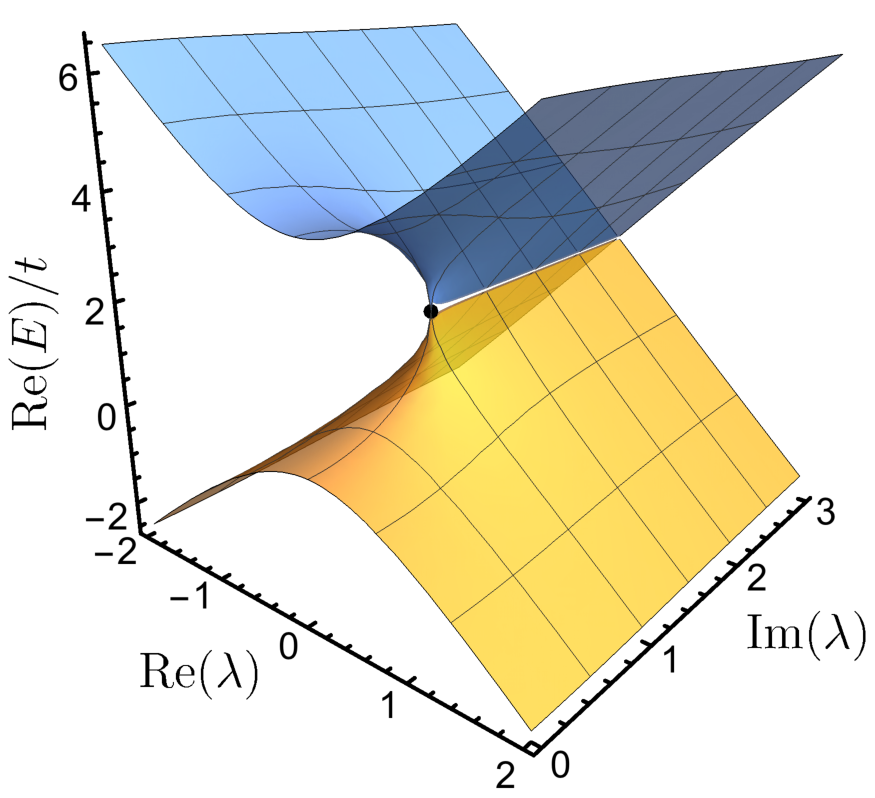
\includegraphics[height=0.65\textwidth]{fig1b}
	\subcaption{\label{subfig:FCI_cplx}}
    \end{subfigure}
	\caption{%
	Exact energies for the Hubbard dimer ($U=4t$) as functions of $\lambda$ on the real axis (\subref{subfig:FCI_real}) and in the complex plane (\subref{subfig:FCI_cplx}).
    Only the interacting closed-shell singlets are plotted in the complex plane, becoming degenerate at the EP (black dot).
    The contour followed around the EP in order to interchange states is also represented.
	\label{fig:FCI}}
\end{figure*}

To illustrate the concepts discussed throughout this article, we will consider the symmetric Hubbard dimer at half filling, \ie\ with two opposite-spin fermions.
Analytically solvable model systems are essential in theoretical chemistry and physics as the simplicity of the
mathematics compared to realistic systems (e.g.\ atoms and molecules) readily allows concepts to be illustrated and new methods to be tested wile retaining much 
of the key physics.

Using the (localised) site basis, the Hilbert space of the Hubbard dimer comprises the four configurations
\begin{align}
& \ket{\Lup \Ldown} &  & \ket{\Lup\Rdown} &  & \ket{\Rup\Ldown} &  & \ket{\Rup\Rdown}
\end{align}
where $\Lsi$ ($\Rsi$) denotes an electron with spin $\sigma$ on the left (right) site.
The exact, or full configuration interaction (FCI), Hamiltonian is then 
\begin{equation}
\label{eq:H_FCI}
	\bH = 
	\begin{pmatrix}
		U &	- t & -  t & 0	\\
	   -  t &  0 &  0 & -  t \\
       -  t &  0 &  0 & -  t \\
        0 & -  t & -  t & U \\
	\end{pmatrix},
\end{equation}
where $t$ is the hopping parameter and $U$ is the on-site Coulomb repulsion.
We refer the interested reader to Refs.~\onlinecite{Carrascal_2015,Carrascal_2018} for more details about this system.
The parameter $U$ controls the strength of the electron correlation.
In the weak correlation regime (small $U$), the kinetic energy dominates and the electrons are delocalised over both sites.
In the large-$U$ (or strong correlation) regime, the electron repulsion term drives the physics and the electrons localise on opposite sites to minimise their Coulomb repulsion. 
This phenomenon is often referred to as Wigner crystallisation. \cite{Wigner_1934}

To illustrate the formation of an EP, we scale the off-diagonal coupling strength by introducing the complex parameter $\lambda$ through the transformation $t\rightarrow \lambda t$.
When $\lambda$ is real, the Hamiltonian~\eqref{eq:H_FCI} is Hermitian with the distinct (real-valued) (eigen)energies
\begin{subequations}
\begin{align}
E_{\mp} &= \frac{1}{2} \qty(U \mp \sqrt{ (4 \lambda t)^2 + U^2 } ),
\label{eq:singletE}
\\
E_{\text{T}} &= 0,
\\
E_{\text{S}} &= U.
\end{align}
\end{subequations}
While the open-shell triplet ($E_{\text{T}}$) and singlet ($E_{\text{S}}$) are independent of $\lambda$, the closed-shell singlet ground state ($E_{-}$) and doubly-excited state ($E_{+}$) couple strongly to form an avoided crossing at $\lambda=0$ (see Fig.~\ref{subfig:FCI_real}).

At non-zero values of $U$ and $t$, these closed-shell singlets can only become degenerate at a pair of complex conjugate points in the complex $\lambda$ plane 
\begin{equation}
\lambda_{\text{EP}} = \pm  \i \frac{U}{4t},
\end{equation}
with energy
\begin{equation}
\label{eq:E_EP}
	E_\text{EP} = \frac{U}{2}.
\end{equation}
These $\lambda$ values correspond to so-called EPs and connect the ground and excited states in the complex plane.
Crucially, the energy surface becomes non-analytic at $\lambda_{\text{EP}}$ and a square-root singularity forms with two branch cuts running along the imaginary axis from $\lambda_{\text{EP}}$  to $\pm \i \infty$ (see Fig.~\ref{subfig:FCI_cplx}).
On the real $\lambda$ axis, these EPs lead to the singlet avoided crossing at $\lambda = \Re(\lambda_{\text{EP}})$.
The ``shape'' of this avoided crossing is related to the magnitude of $\Im(\lambda_{\text{EP}})$, with smaller values giving a ``sharper'' interaction.

Remarkably, the existence of these square-root singularities means that following a complex contour around an EP in the complex $\lambda$ plane will interconvert the closed-shell ground and excited states (see Fig.~\ref{subfig:FCI_cplx}).
This behaviour can be seen by expanding the radicand in Eq.~\eqref{eq:singletE} as a Taylor series around $\lambda_{\text{EP}}$ to give
\begin{equation}
E_{\pm} \approx E_{\text{EP}} \pm \sqrt{32t^2 \lambda_{\text{EP}}} \sqrt{\lambda - \lambda_{\text{EP}}}.
\end{equation}
Parametrising the complex contour as $\lambda(\theta) = \lambda_{\text{EP}} + R \exp(\i \theta)$ gives the continuous energy pathways 
\begin{equation}
E_{\pm} \qty(\theta) \approx E_{\text{EP}} \pm \sqrt{32t^2 \lambda_{\text{EP}} R}\, \exp(\i \theta/2)
\end{equation}
such that $E_{\pm}(2\pi)  = E_{\mp}(0)$ and $E_{\pm}(4\pi)  = E_{\pm}(0)$.
As a result, completely encircling an EP leads to the interconversion of the two interacting states, while a second complete rotation returns the two states to their original energies.
Additionally, the wave functions pick up a geometric phase in the process, and four complete loops are required to recover their starting forms.\cite{MoiseyevBook}

%%%%%%%%%%%%%%%%%%%%%%%%%%%%%%
\section{Perturbation theory}
%%%%%%%%%%%%%%%%%%%%%%%%%%%%%%

%============================================================%
\subsection{Rayleigh-Schr\"odinger perturbation theory}
%============================================================%

Within the Born-Oppenheimer approximation, the exact molecular Hamiltonian with $\Ne$ electrons and 
$\Nn$ (clamped) nuclei is defined as
\begin{equation}\label{eq:ExactHamiltonian}
    \hH = 
    - \frac{1}{2} \sum_{i}^{\Ne} \grad_i^2 
    - \sum_{i}^{\Ne} \sum_{A}^{\Nn} \frac{Z_A}{\abs{\vb{r}_i-\vb{R}_A}} 
    + \sum_{i<j}^{\Ne}\frac{1}{\abs{\vb{r}_i-\vb{r}_j}},
\end{equation}
where $\vb{r}_i$ defines the position of the $i$-th electron, and $\vb{R}_{A}$ and $Z_{A}$ are the position
and charge of the $A$-th nucleus respectively.
The first term represents the kinetic energy of the electrons, while 
the two following terms account for the electron-nucleus attraction and the electron-electron repulsion.
Atomic units are used unless otherwise stated.

% EXACT SCHRODINGER EQUATION
The exact many-electron wave function $\Psi$ corresponds to the solution of the (time-independent)
Schr\"{o}dinger equation
\begin{equation} 
	\hH\Psi = E \Psi,
    \label{eq:SchrEq}
\end{equation} 
with the eigenvalue $E$ providing the exact energy.
Exact solutions to Eq.~\eqref{eq:SchrEq} are only possible in the simplest of systems, such as 
the one-electron hydrogen atom. 
In practice, one of the most common approximations involves
a perturbative expansion of the energy.
% SUMMARY OF RS-PT
Within Rayleigh-Schr\"odinger perturbation theory, the time-independent Schr\"odinger equation 
is recast as 
\begin{equation} 
	\hH(\lambda) \Psi(\lambda) 
    = \qty(\hH^{(0)} + \lambda \hV ) \Psi(\lambda) 
    = E(\lambda) \Psi(\lambda),
    \label{eq:SchrEq-PT}
\end{equation}
where $\hH^{(0)}$ is a zeroth-order Hamiltonian and $\hV = \hH - \hH^{(0)}$ represents the perturbation operator.
Expanding the wave function and energy as power series in $\lambda$ as 
\begin{subequations}
\begin{align}
    \Psi(\lambda) &= \sum_{k=0}^{\infty} \lambda^{k}\,\Psi^{(k)} 
    \label{eq:psi_expansion}
    \\
    E(\lambda) &= \sum_{k=0}^{\infty} \lambda^{k}\,E^{(k)},
    \label{eq:E_expansion}
\end{align}
\end{subequations}
solving the corresponding perturbation equations up to a given order $k$, and
setting $\lambda = 1$ then yields approximate solutions to Eq.~\eqref{eq:SchrEq}.

% MATHEMATICAL REPRESENTATION
Mathematically, Eq.~\eqref{eq:E_expansion} corresponds to a Taylor series expansion of the exact energy
around the reference system $\lambda = 0$.
The energy of the target ``physical'' system is recovered at the point $\lambda = 1$.
However, like all series expansions, the Eq.~\eqref{eq:E_expansion} has a radius of convergence $\rc$. 
When $\rc \le 1$, the Rayleigh--Sch\"{r}odinger expansion will diverge
for the physical system.
The value of $\rc$ can vary significantly between different systems and strongly depends on the particular decomposition
of the reference and perturbation Hamiltonians in Eq.~\eqref{eq:SchrEq-PT}.\cite{Mihalka_2017b}

% LAMBDA IN THE COMPLEX PLANE
From complex-analysis, the radius of convergence for the energy can be obtained by looking for the 
singularities of $E(\lambda)$ in the complex $\lambda$ plane.
This property arises from the following theorem: \cite{Goodson_2012}
\begin{quote}
\it
``The Taylor series about a point $z_0$ of a function over the complex $z$ plane will converge at a value $z_1$ 
if the function is non-singular at all values of $z$ in the circular region centred at $z_0$ with radius $\abs{z_1-z_0}$. 
If the function has a singular point $z_s$ such that $\abs{z_s-z_0} < \abs{z_1-z_0}$, 
then the series will diverge when evaluated at $z_1$.''
\end{quote}
As a result, the radius of convergence for a function is equal to the distance from the origin of the closest singularity
in the complex plane.
For example, the simple function
\begin{equation} \label{eq:DivExample}
	f(x)=\frac{1}{1+x^4}.
\end{equation}
is smooth and infinitely differentiable for $x \in \mathbb{R}$, and one might expect that its Taylor series expansion would 
converge in this domain.
However, this series diverges $x \ge 1$.
This divergence occurs because $f(x)$ has four singularities in the complex 
($\e^{\i\pi/4}$, $\e^{-\i\pi/4}$, $\e^{\i3\pi/4}$, and $\e^{-\i3\pi/4}$) with a modulus equal to $1$, demonstrating
that complex singularities are essential to fully understand the series convergence on the real axis.\cite{BenderBook}

The radius of convergence for the perturbation series is therefore dictated by the magnitude $\abs{\lambda_0}$ of the
singularity in $E(\lambda)$ that is closest to the origin.
Like the exact system in Section~\ref{sec:example}, the perturbation energy $E(\lambda)$ represents
a ``one-to-many'' function with the output elements representing an approximation to both the ground and excited states.
The most common singularities on $E(\lambda)$ therefore correspond to non-analytic EPs in the complex 
$\lambda$ plane where two states become degenerate.
Later we will demonstrate how the choice of reference Hamiltonian controls the position of these EPs, and 
ultimately determines the convergence properties of the perturbation series.


Practically, to locate EPs in a more complicated systems, one must simultaneously solve
\begin{subequations}
\begin{align}
	\label{eq:PolChar}
	\det[E\hI-\hH(\lambda)] & = 0,
	\\ 
	\label{eq:DPolChar}
	\pdv{E}\det[E\hI-\hH(\lambda)] & = 0,
\end{align}
\end{subequations}
where $\hI$ is the identity operator.\cite{Cejnar_2007}
Equation \eqref{eq:PolChar} is the well-known secular equation providing the (eigen)energies of the system. 
If the energy is also solution of Eq.~\eqref{eq:DPolChar}, then this energy value is at least two-fold degenerate. 
These degeneracies can be conical intersections between two states with different symmetries 
for real values of $\lambda$,\cite{Yarkony_1996} or EPs between two states with the 
same symmetry for complex values of $\lambda$.


%============================================================%
\subsection{The Hartree-Fock Hamiltonian}
%============================================================%

% SUMMARY OF HF
In the Hartree-Fock (HF) approximation, the many-electron wave function is approximated as a single Slater determinant $\Psi^{\text{HF}}(\vb{x}_1,\ldots,\vb{x}_N)$, where $\vb{x} = (\sigma,\vb{r})$ is a composite vector gathering spin and spatial coordinates.
This Slater determinant is defined as an antisymmetric combination of $\Ne$ (real-valued) occupied one-electron spin-orbitals $\phi_p(\vb{x})$, which are, by definition, eigenfunctions of the one-electron Fock operator 
\begin{equation}\label{eq:FockOp}
    \Hat{f}(\vb{x}) \phi_p(\vb{x}) = \qty( \Hat{h}(\vb{x}) + \Hat{v}_\text{HF}(\vb{x}) ) \phi_p(\vb{x}) = \epsilon_p \phi_p(\vb{x}).
\end{equation}
Here the core Hamiltonian is
\begin{equation}
	\Hat{h}(\vb{x}) = -\frac{\grad^2}{2} + \sum_{A}^{M} \frac{Z_A}{\abs{\vb{r}-\vb{R}_A}}
\end{equation}
and
\begin{equation}
    \Hat{v}_\text{HF}(\vb{x}) = \sum_i^{N} \qty( \Hat{J}_i(\vb{x}) - \Hat{K}_i(\vb{x}) )
\end{equation}
is the HF mean-field electron-electron potential with 
\begin{subequations}
\begin{gather}
	\label{eq:CoulOp}
    \Hat{J}_i(\vb{x})\phi_j(\vb{x})=\qty(\int \phi_i(\vb{x}')\frac{1}{\abs{\vb{r} - \vb{r}'}}\phi_i(\vb{x}') \dd\vb{x}' ) \phi_j(\vb{x}),
	\\
	\label{eq:ExcOp}
\Hat{K}_i(\vb{x})\phi_j(\vb{x})=\qty(\int \phi_i(\vb{x}')\frac{1}{\abs{\vb{r} - \vb{r}'}}\phi_j(\vb{x}') \dd\vb{x}')\phi_i(\vb{x}),
\end{gather}
\end{subequations}
defining the Coulomb and exchange operators (respectively) in the spin-orbital basis.\cite{SzaboBook}
The HF energy is then defined as 
\begin{equation}
    \label{eq:E_HF}
    E_\text{HF} = \hugh{\frac{1}{2} \sum_i^{N} \Big( h_i + f_i \Big)},
	%E_\text{HF} = \sum_i^{N} h_i + \frac{1}{2} \sum_{ij}^{N} \qty( J_{ij} - K_{ij} ),
\end{equation}
with the corresponding matrix elements
\begin{align}
	h_i = \mel{\phi_i}{\Hat{h}}{\phi_i}
    \quad \text{and} \quad
    \hugh{f_i = \mel{\phi_i}{\Hat{f}}{\phi_i}.}
	%J_{ij} & = \mel{\phi_i}{\Hat{J}_j}{\phi_i},
	%&
	%K_{ij} & = \mel{\phi_i}{\Hat{K}_j}{\phi_i}.
\end{align}
The optimal HF wave function is identified by using the variational principle to minimise the HF energy.
For any system with more than one electron, the resulting Slater determinant is not an eigenfunction of the exact Hamiltonian $\hH$. 
However, it is by definition an eigenfunction of the approximate many-electron HF Hamiltonian constructed 
from the one-electron Fock operators as
\begin{equation}\label{eq:HFHamiltonian}
	\hH_{\text{HF}} = \sum_{i} f(\vb{x}_i).
\end{equation}
From hereon, $i$ and $j$ denote occupied orbitals, $a$ and $b$ denote unoccupied (or virtual) orbitals, while $p$, $q$, $r$, and $s$ denote arbitrary orbitals.

% BRIEF FLAVOURS OF HF
In the most flexible variant of real HF theory (generalised HF) the one-electron orbitals can be complex-valued
and contain a mixture of spin-up and spin-down components.\cite{Mayer_1993}
However, the application of HF with some level of constraint on the orbital structure is far more common.
Forcing the spatial part of the orbitals to be the same for spin-up and spin-down electrons leads to restricted HF (RHF) theory, while allowing different for different spins leads to the so-called unrestricted HF (UHF) approach.
The advantage of the UHF approximation is its ability to correctly describe strongly correlated systems, 
such as the dissociation of the hydrogen dimer.\cite{Coulson_1949}
However, by allowing different orbitals for different spins, the UHF is no longer required to be an eigenfunction of 
the total spin $\hat{\mathcal{S}}^2$ operator, leading to ``spin-contamination'' in the wave function.

%
%The spatial part of the RHF wave function is then
%\begin{equation}\label{eq:RHF_WF}
%	\Psi_{\text{RHF}}(\theta_1,\theta_2) = Y_0(\theta_1) Y_0(\theta_2),
%\end{equation}
%where $\theta_i$ is the polar angle of the $i$th electron and $Y_{\ell}(\theta)$ is a zonal spherical harmonic. 
%Because $Y_0(\theta) = 1/\sqrt{4\pi}$, it is clear that the RHF wave function yields a uniform one-electron density.
%

%%% FIG 2 (?) %%%
% HF energies as a function of U/t
%%%%%%%%%%%%%%%%%
\begin{figure}
    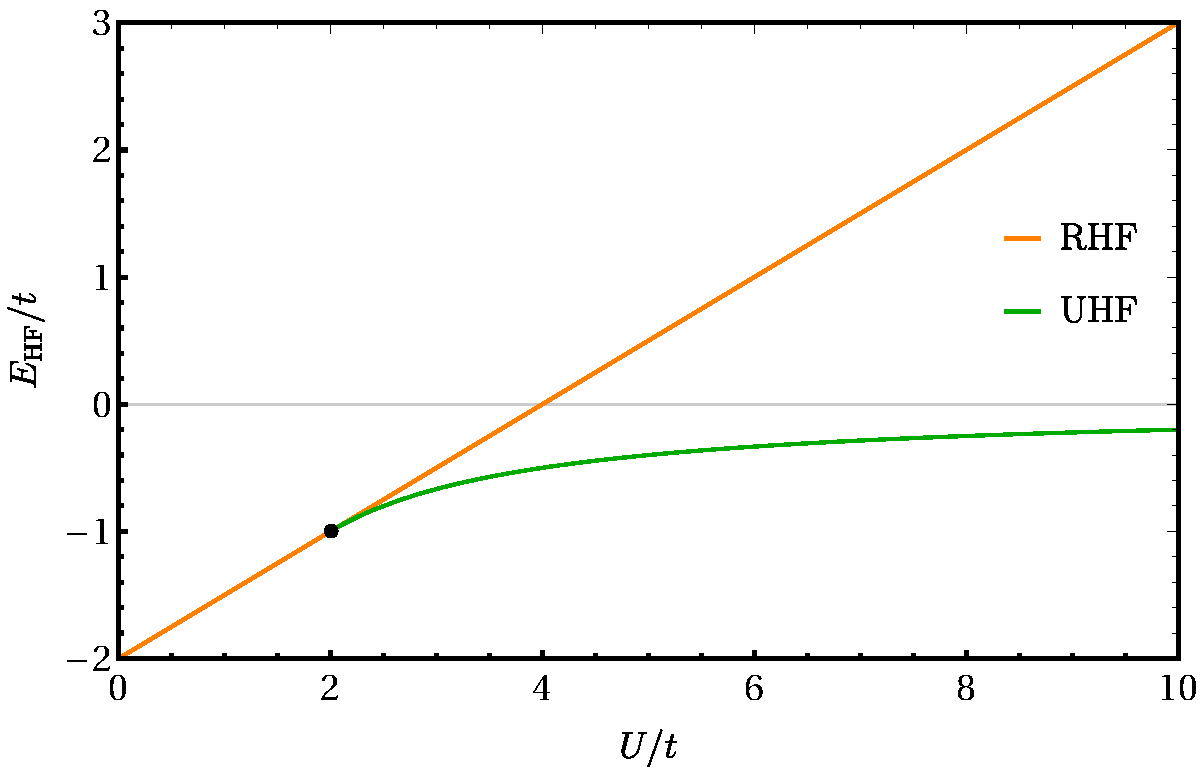
\includegraphics[width=\linewidth]{HF_real.pdf}
    \caption{\label{fig:HF_real}
    RHF and UHF energies as a function of the correlation strength $U/t$. 
    The symmetry-broken UHF solution emerges at the coalescence point $U=2t$ (black dot) known as the Coulson-Fischer point.}
\end{figure}
%%%%%%%%%%%%%%%%%

Returning to the Hubbard dimer, the UHF energy can be parametrised in terms of two rotation angles $\ta$ and $\tb$ as
\begin{equation}
E_\text{HF}(\ta, \tb) = -t \qty( \sin \ta + \sin \tb ) + \frac{U}{2} \qty( 1 + \cos \ta \cos \tb ),
\end{equation}
where we have introduced bonding $\mathcal{B}^{\sigma}$ and anti-bonding $\mathcal{A}^{\sigma}$ molecular orbitals for 
the spin-$\sigma$ electrons as
\begin{align}
    \mathcal{B}^{\sigma} & = \hphantom{-} \cos(\frac{\theta_\sigma}{2}) \Lsi + \sin(\frac{\theta_\sigma}{2}) \Rsi,
	\\
	\mathcal{A}^{\sigma} & = - \sin(\frac{\theta_\sigma}{2}) \Lsi + \cos(\frac{\theta_\sigma}{2}) \Rsi
\end{align}
In the weak correlation regime $0 \le U \le 2t$, the angles which minimise the HF energy, 
\ie, $\pdv*{E_\text{HF}}{\theta_\sigma} = 0$, are 
\begin{equation}
	\ta^\text{RHF} = \tb^\text{RHF} = \pi/2,
\end{equation}
giving the symmetry-pure molecular orbitals
\begin{align}
	\mathcal{B}_\text{RHF}^{\sigma} & = \frac{\Lsi + \Rsi}{\sqrt{2}},
	&
	\mathcal{A}_\text{RHF}^{\sigma} & = \frac{\Lsi - \Rsi}{\sqrt{2}},
\end{align}
and the ground-state RHF energy (Fig.~\ref{fig:HF_real})
\begin{equation}
	E_\text{RHF} \equiv E_\text{HF}(\ta^\text{RHF}, \tb^\text{RHF}) = -2t + \frac{U}{2}
\end{equation}
However, in the strongly correlated regime $U>2t$, the closed-shell restriction on the orbitals prevents RHF from 
correctly modelling the physics of the system with the two electrons on opposing sites.

%%% FIG 3 (?) %%%
% Analytic Continuation of HF
%%%%%%%%%%%%%%%%%
\begin{figure*}[t]
	\begin{subfigure}{0.49\textwidth}
    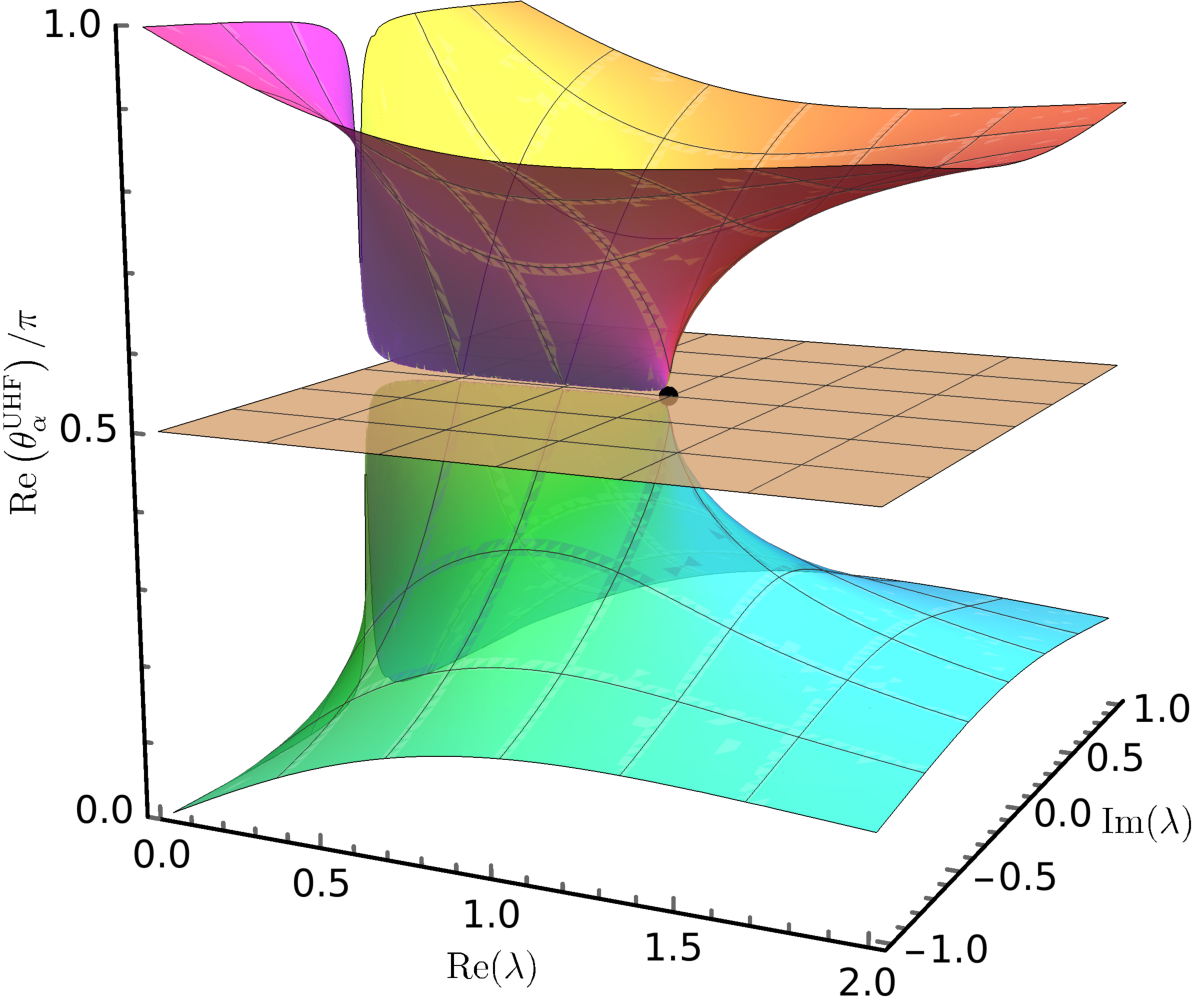
\includegraphics[height=0.65\textwidth,trim={0pt 0pt 0pt -35pt},clip]{HF_cplx_angle}
	\subcaption{\label{subfig:UHF_cplx_angle}}
    \end{subfigure}
	\begin{subfigure}{0.49\textwidth}
	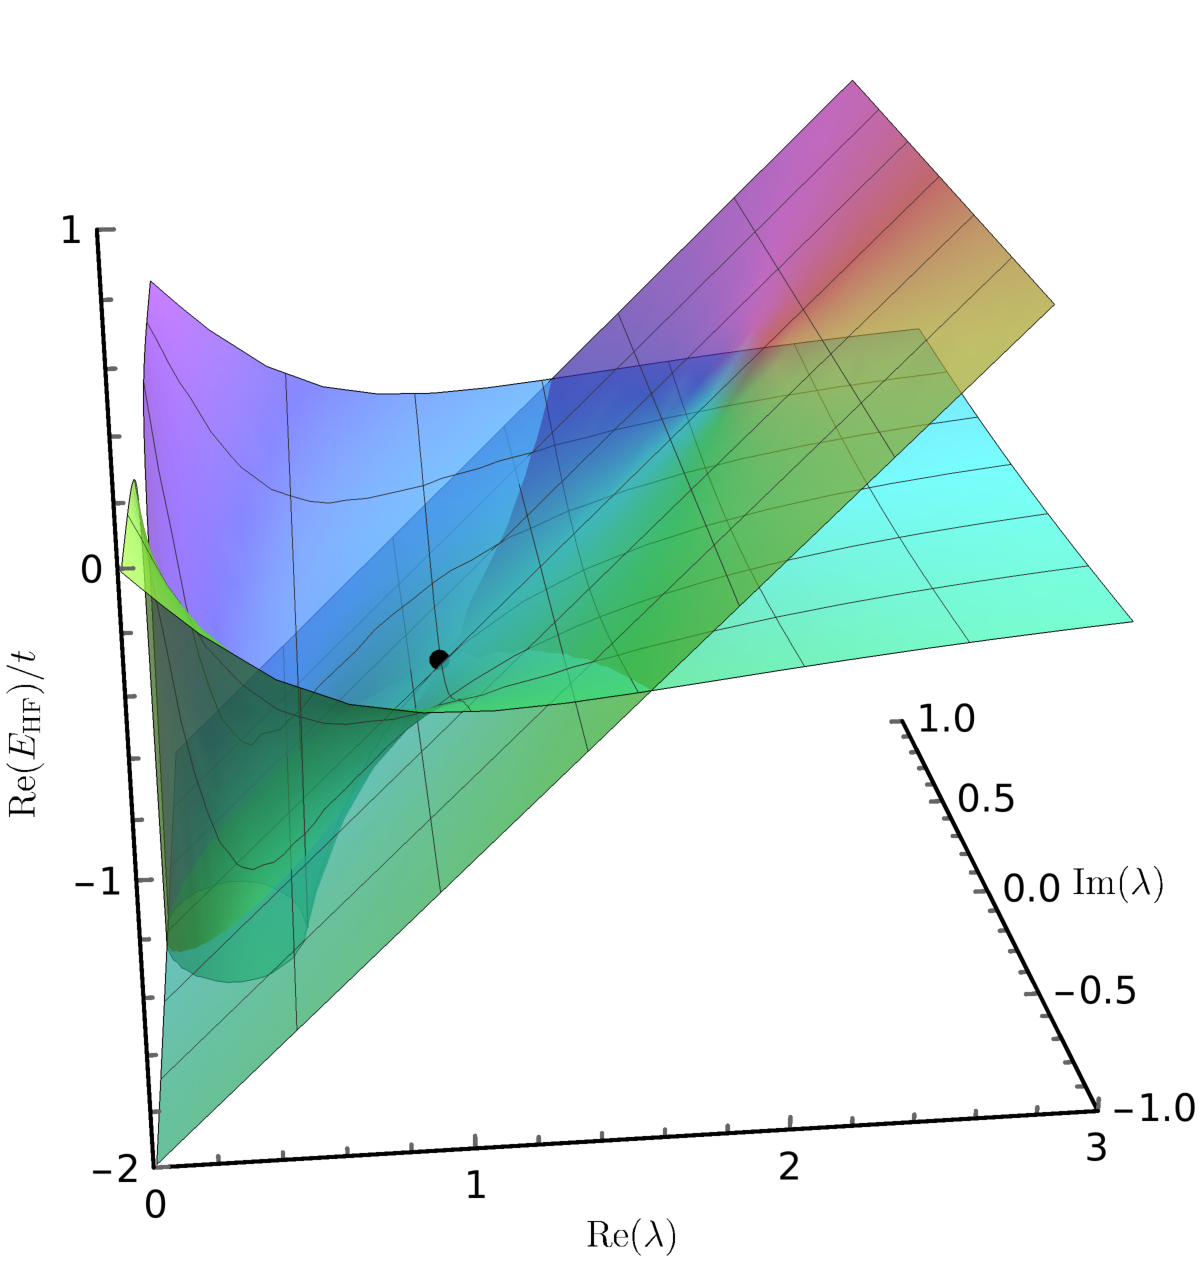
\includegraphics[height=0.65\textwidth]{HF_cplx_energy}
	\subcaption{\label{subfig:UHF_cplx_energy}}
    \end{subfigure}
	\caption{%
    (\subref{subfig:UHF_cplx_angle}) Real component of the UHF angle $\ta^{\text{UHF}}$ for $\lambda \in \bbC$.
    Symmetry-broken solutions correspond to individual sheets and become equivalent at 
    the \textit{quasi}-EP $\lambda_{\text{c}}$ (black dot).
    The RHF solution is independent of $\lambda$, giving constant plane at $\pi/2$.
    (\subref{subfig:UHF_cplx_energy}) The corresponding HF energy surfaces show a non-analytic 
    point at the \textit{quasi}-EP.
	\label{fig:HF_cplx}}
\end{figure*}
%%%%%%%%%%%%%%%%%

As the on-site repulsion is increased from 0, the HF approximation reaches a critical value at $U=2t$ where a symmetry-broken 
UHF solution appears with a lower energy than the RHF one.
This critical point is analogous to the infamous Coulson--Fischer point identified in the hydrogen dimer.\cite{Coulson_1949}
For $U \ge 2t$, the optimal orbital rotation angles for the UHF orbitals become
\begin{align}
    \ta^\text{UHF} & = \arctan (-\frac{2t}{\sqrt{U^2 - 4t^2}}),
    \label{eq:ta_uhf}
	\\
    \tb^\text{UHF} & = \arctan (+\frac{2t}{\sqrt{U^2 - 4t^2}}),
    \label{eq:tb_uhf}
\end{align}
with the corresponding UHF ground-state energy (Fig.~\ref{fig:HF_real})
\begin{equation}
	E_\text{UHF} \equiv E_\text{HF}(\ta^\text{UHF}, \tb^\text{UHF}) = - \frac{2t^2}{U}.
\end{equation}
Time-reversal symmetry dictates that this UHF wave function must be degenerate with its spin-flipped pair, obtained 
by swapping $\ta^{\text{UHF}}$ and $\tb^{\text{UHF}}$ in Eqs.~\eqref{eq:ta_uhf} and \eqref{eq:tb_uhf}.
Note that the RHF wave function remains a genuine solution of the HF equations for $U \ge 2t$, but corresponds to a saddle point 
of the HF energy rather than a minimum.

%============================================================%
\subsection{Self-consistency as a perturbation} %OR {Complex adiabatic connection}
%============================================================%

% INTRODUCE PARAMETRISED FOCK HAMILTONIAN
The inherent non-linearity in the Fock eigenvalue problem arises from self-consistency 
in the HF approximation, and is usually solved through an iterative approach.\cite{SzaboBook}
Alternatively, the non-linear terms arising from the Coulomb and exchange operators can 
be considered as a perturbation from the core Hamiltonian by introducing the
transformation $U \rightarrow \lambda\, U$, giving the parametrised Fock operator 
\begin{equation}
    \Hat{f}_{\lambda}(\vb{x}) = \Hat{h}(\vb{x}) + \lambda\, \Hat{v}_\text{HF}(\vb{x}).
\end{equation}
The orbitals in the reference problem $\lambda=0$ correspond to the symmetry-pure eigenfunctions of the one-electron core
Hamiltonian, while self-consistent solutions at $\lambda = 1$ represent the orbitals of the true HF solution.

% INTRODUCE COMPLEX ANALYTIC-CONTINUATION
For real $\lambda$, the self-consistent HF energies at given (real) $U$ and $t$ values
in the Hubbard dimer directly mirror the energies shown in Fig.~\ref{fig:HF_real}, 
with coalesence points at 
\begin{equation}
    \lambda_{\text{c}} = \pm \frac{2t}{U}.
    \label{eq:scaled_fock}
\end{equation}
In contrast, when $\lambda$ becomes complex, the HF equations become non-Hermitian and 
each HF solutions can be analytically continued for all $\lambda$ values using
the holomorphic HF approach.\cite{Hiscock_2014,Burton_2016,Burton_2018}
Remarkably, the coalescence point in this analytic continuation emerges as a 
\textit{quasi}-EP on the real $\lambda$ axis (Fig.~\ref{fig:HF_cplx}), where
the different HF solutions become equivalent but not self-orthogonal.\cite{Burton_2019}
By analogy with perturbation theory, the regime where this \textit{quasi}-EP occurs 
within $\lambda_{\text{c}} \le 1$ can be interpreted as an indication that 
the symmetry-pure reference orbitals no longer provide a qualitatively 
accurate representation for the true HF ground state at $\lambda = 1$.
For example, in the Hubbard dimer with $U > 2t$, one finds $\lambda_{\text{c}} < 1$ and the symmetry-pure orbitals
do not provide a good representation of the HF ground state.
In contrast, $U < 2t$ yields $\lambda_{\text{c}} > 1$ and corresponds to
the regime where the HF ground state is correctly represented by symmetry-pure orbitals.

% COMPLEX ADIABATIC CONNECTION
We have recently shown that the complex scaled Fock operator Eq.~\eqref{eq:scaled_fock}
also allows states of different symmetries to be interconverted by following a well-defined
contour in the complex $\lambda$-plane.\cite{Burton_2019}
In particular, by slowly varying $\lambda$ in a similar (yet different) manner
to an adiabatic connection in density-functional theory,\cite{Langreth_1975,Gunnarsson_1976,Zhang_2004} 
a ground-state wave function can be ``morphed'' into an excited-state wave function 
via a stationary path of HF solutions.
This novel approach to identifying excited-state wave functions demonstrates the fundamental 
role of \textit{quasi}-EPs in determining the behaviour of the HF approximation.

%\titou{In a recent paper, \cite{Burton_2019} using holomorphic Hartree-Fock (h-HF) \cite{Hiscock_2014,Burton_2018,Burton_2016} as an analytic continuation of conventional HF theory, we have demonstrated, on a simple model, that one can interconvert states of different symmetries and natures by following well-defined contours in the complex $\lambda$-plane, where $\lambda$ is the strength of the electron-electron interaction (see Fig.~\ref{fig:iAC}).
%In particular, by slowly varying $\lambda$ in a similar (yet different) manner to an adiabatic connection in density-functional theory, \cite{Langreth_1975,Gunnarsson_1976,Zhang_2004} one can ``morph'' a ground-state wave function into an excited-state wave function via a stationary path of HF solutions. \cite{Seidl_2018}
%In such a way, we could obtain a doubly-excited state wave function starting from the ground state wave function, a process which is not as easy as one might think. \cite{Gilbert_2008,Thom_2008,Shea_2018}
%One of the fundamental discovery we made was that Coulson-Fischer points (where multiple symmetry-broken solutions coalesce) play a central role and can be classified as \textit{quasi}-exceptional points, as the wave functions do not become self-orthogonal.
%The findings reported in Ref.~\onlinecite{Burton_2019} represent the very first study of non-Hermitian quantum mechanics for the exploration of multiple solutions at the HF level. 
%It perfectly illustrates the deeper topology of electronic states revealed using a complex-scaled electron-electron interaction.
%Through the introduction of non-Hermiticity, we have provided a more general framework in which the complex and diverse characteristics of multiple solutions can be explored and understood.}

%=====================================================%
\subsection{M{\o}ller-Plesset perturbation theory}
%=====================================================%

In electronic structure, the HF Hamiltonian \eqref{eq:HFHamiltonian} is often used as the zeroth-order Hamiltonian
to define M\o{}ller--Plesset (MP) perturbation theory.\cite{Moller_1934}
This approach can recover a large proportion of the electron correlation energy,\cite{Lowdin_1955} 
and provides the foundation for numerous post-HF approximations.
With the MP partitioning, the parametrised perturbation Hamiltonian becomes
\begin{multline}\label{eq:MPHamiltonian}
    \hH(\lambda) = 
    \sum_{i}^{N} \Bigg( 
    -\frac{\grad_i^2}{2} 
    - \sum_{A}^{M} \frac{Z_A}{\abs{\vb{r}_i-\vb{R}_A}} 
    \\
    + (1-\lambda) v^{\text{HF}}(\vb{x}_i) 
    + \lambda\sum_{i<j}^{N}\frac{1}{\abs{\vb{r}_i-\vb{r}_j}} 
    \Bigg).
\end{multline}
Any set of orbitals can be used to define the HF Hamiltonian, although usually either the RHF or UHF orbitals are chosen to 
define the RMP or UMP series respectively.
The MP energy at a given order $n$ (\ie, MP$n$) is then defined as
\begin{equation}
	E_{\text{MP}n}= \sum_{k=0}^n E_{\text{MP}}^{(k)},
\end{equation}
where $E_{\text{MP}}^{(k)}$ is the $k$th-order MP correction and 
\begin{equation}
E_{\text{MP1}} =  E_{\text{MP}}^{(0)} + E_{\text{MP}}^{(1)} = E_\text{HF}.
\end{equation}
The second-order MP2 energy is given by
\begin{equation}\label{eq:EMP2}
	E_{\text{MP2}} = \frac{1}{4} \sum_{ij} \sum_{ab} \frac{\abs{\mel{ij}{}{ab}}^2}{\epsilon_i + \epsilon_j - \epsilon_a - \epsilon_b},
\end{equation}
where $\mel{pq}{}{rs} = \braket{pq}{rs} - \braket{pq}{sr}$ are the anti-symmetrised two-electron integrals
in the molecular spin-obital basis\cite{Gill_1994}
\begin{equation}
	\braket{pq}{rs} 
    = \iint \dd\vb{x}_1\dd\vb{x}_2
    \frac{\phi^{*}_p(\vb{x}_1)\phi^{*}_q(\vb{x}_2)\phi^{\vphantom{*}}_r(\vb{x}_1)\phi^{\vphantom{*}}_s(\vb{x}_2)}%
      {\abs{\vb{r}_1 - \vb{r}_2}}.
\end{equation}

\hugh{While most practical calculations usually consider only the MP2 or MP3 approximations, higher order terms can 
easily be computed to understand the convergence of the MP$n$ series.\cite{Handy_1985}}
\textit{A priori}, there is no guarantee that this series will provide the smooth convergence that is desirable for a
systematically improvable theory.
\hugh{In fact, when the reference HF wave function is a poor approximation to the exact wave function, 
for example in multi-configurational systems, MP theory can yield highly oscillitory, 
slowly convergent, or catastrophically divergent results.\cite{Gill_1986,Gill_1988,Handy_1985,Lepetit_1988,Leininger_2000}
Furthermore, the convergence properties of the MP series can depend strongly on the choice of restricted or
unrestricted reference orbitals.}

% HGAB: I don't think this parapgrah tells us anything we haven't discussed before
%A convenient way to investigate the convergence properties of the MP series is to analytically continue the coupling parameter $\lambda$ into the complex variable. 
%By doing so, the Hamiltonian and the energy become complex-valued functions of $\lambda$, 
%and the energy becomes a multivalued function on $K$ Riemann sheets (where $K$ is the number of basis functions).
%As mentioned above, by searching the singularities of the function $E(\lambda)$, one can get information on the convergence properties of the MP series. 
%These singularities of the energy function are exactly the EPs connecting the electronic states as mentioned in Sec.~\ref{sec:intro}. 
%The direct computation of the terms of the series is quite manageable up to fourth order in perturbation, while the fifth and sixth order in perturbation can still be obtained but at a rather high cost. \cite{JensenBook}
%In order to better understand the behavior of the MP series and how it is connected to the singularity structure, we have to access high-order terms. 
%For small systems, one can access the whole terms of the series using full configuration interaction (FCI). 
%If the Hamiltonian $H(\lambda)$ is diagonalized in the FCI space, one gets the exact energies (in this finite Hilbert space) and the Taylor expansion with respect to $\lambda$ allows to access the MP perturbation series at any order.

To illustrate the behaviour of the RMP and UMP series, we can again consider the Hubbard dimer.
Using the ground-state RHF reference orbitals leads to the RMP Hamiltonian
\begin{widetext}
\begin{equation}
\label{eq:H_RMP}
\bH_\text{RMP}\hugh{\qty(\lambda)} = 
	\begin{pmatrix}
		-2t + U - \lambda U/2	&	0					&	0					&	\lambda U/2	\\
		0						&	U - \lambda U/2 	&	\lambda U/2			&	0	\\
		0						&	\lambda U/2			&	U - \lambda U/2 	&	0	\\
		\lambda U/2 			&	0 					&	0					&	2t + U - \lambda U/2	\\
	\end{pmatrix},
\end{equation}
\end{widetext}
which yields the ground-state energy 
\begin{equation}
	\label{eq:E0MP}
	E_{-}(\lambda) = U - \frac{\lambda U}{2} - \frac{1}{2} \sqrt{(4t)^2 + \lambda ^2 U^2}.
\end{equation}
From this expression, the EPs can be identified as $\lep = \pm \i 4t / U$,
giving the radius of convergence
\begin{equation}
    \rc = \qty|\frac{4t}{U}|.
\end{equation}
These EPs are identical the the exact EPs discussed in Sec.~\ref{sec:example}.
The Taylor expansion of the RMP energy can then be evaluated to obtain the $n$th order MP correction
\begin{equation}
	E_\text{RMP}^{(k)} = U \delta_{0,k} - \frac{1}{2} \frac{U^k}{(4t)^{k-1}} \mqty( 1/2 \\ k/2).
\end{equation}
%with 
%\begin{equation}
%	E_{\text{MP}n}(\lambda) = \sum_{k=0}^n E_\text{MP}^{(k)} \lambda^k.
%\end{equation}

\hugh{The RMP series is convergent for $U = 3.5\,t$ with $\rc > 1$, as illustrated for the individual terms at each order
of perturbation in Fig.~\ref{subfig:RMP_cvg}.
In contrast, for $U = 4.5t$ one finds $\rc < 1$, and the RMP series becomes divergent.
The corresponding Riemann surfaces for $U = 3.5\,t$ and $4.5\,t$ are shown in Figs.~\ref{subfig:RMP_3.5} and 
\ref{subfig:RMP_4.5} respectively, with the single EP at $\lep$ (black dot) and the radius of convergence indicated
by the vertical cylinder of unit radius.
For the divergent case, the $\lep$ lies inside this cylinder of convergence, while in the convergent case $\lep$ lies
outside this cylinder.
In both cases, the EP connects the ground state with the doubly-excited state, and thus the convergence behaviour
for the two states using the ground state RHF orbitals is identical.
The convergent and divergent series start to differ at fourth order, corresponding to the lowest-order contribution
from the single excitations.\cite{Lepetit_1998}
This divergent behaviour might therefore be attributed to the need for the single excitations to focus on correcting
the structure of the reference orbitals rather than capturing the correlation energy.
} 

%%% FIG 2 %%%
\begin{figure*}
	\begin{subfigure}{0.32\textwidth}
	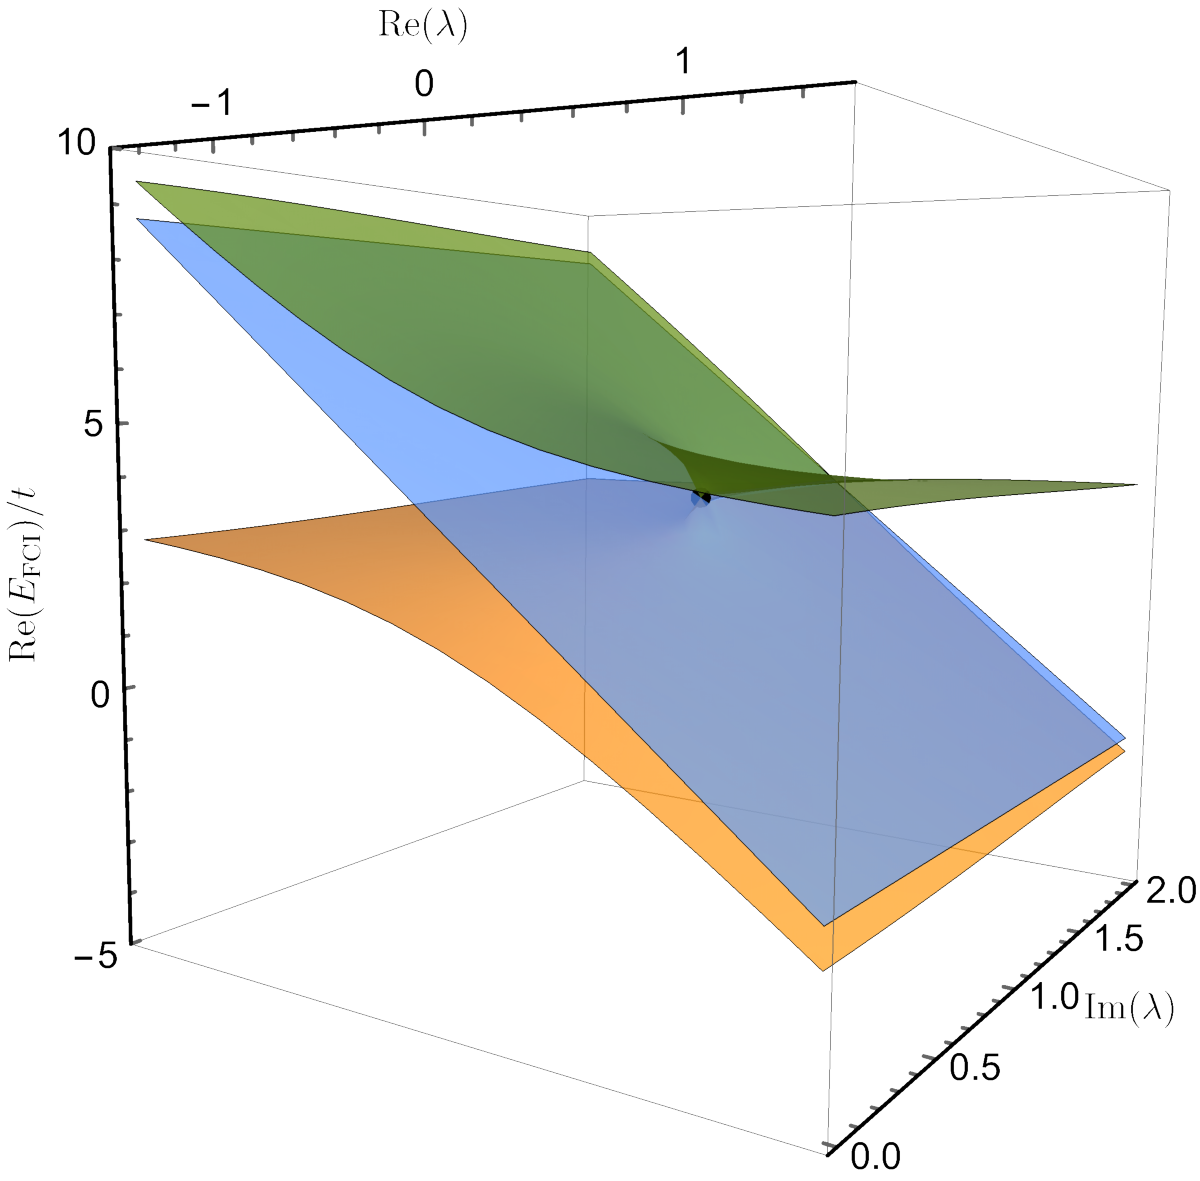
\includegraphics[height=0.75\textwidth]{fig2a}	
		\subcaption{\label{subfig:RMP_3.5} $U/t = 3.5$}
    \end{subfigure}
    %
    \begin{subfigure}{0.32\textwidth}
	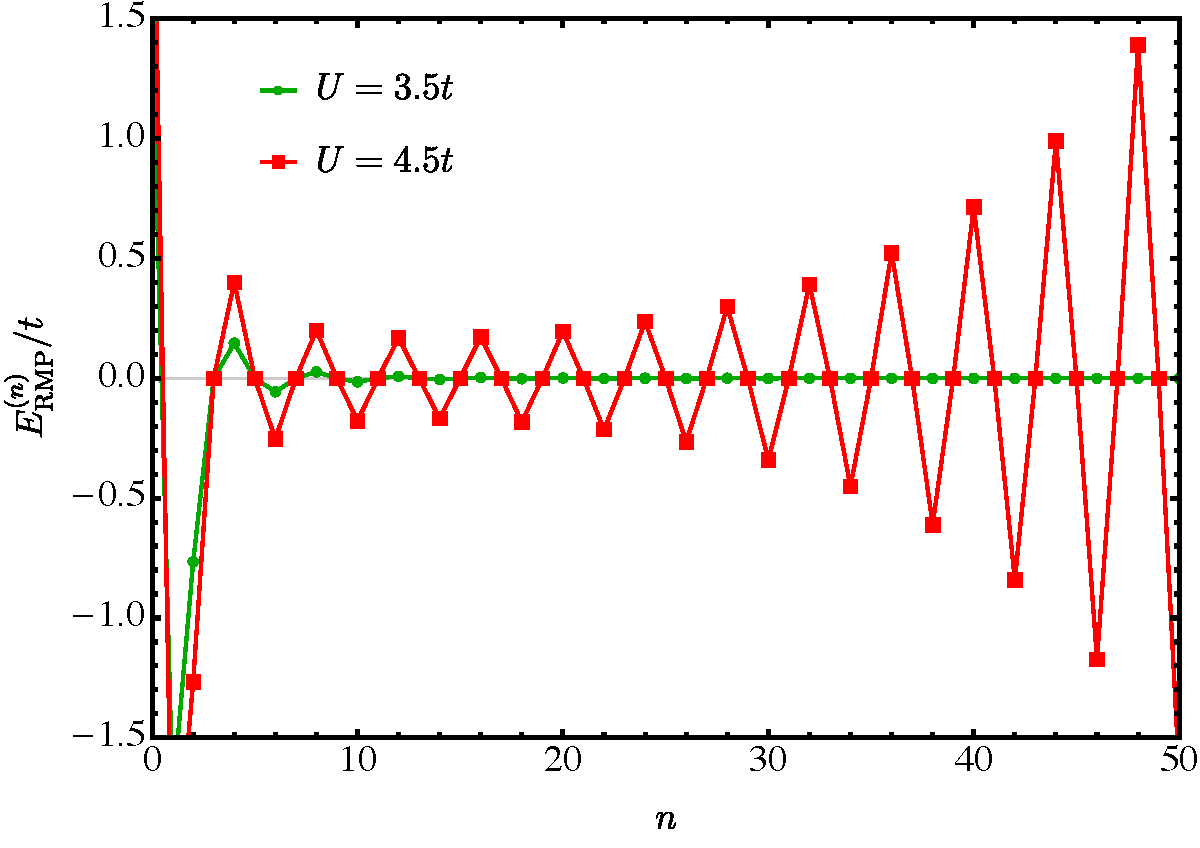
\includegraphics[height=0.75\textwidth]{fig2b}
		\subcaption{\label{subfig:RMP_cvg}}
    \end{subfigure}
    %
    \begin{subfigure}{0.32\textwidth}
	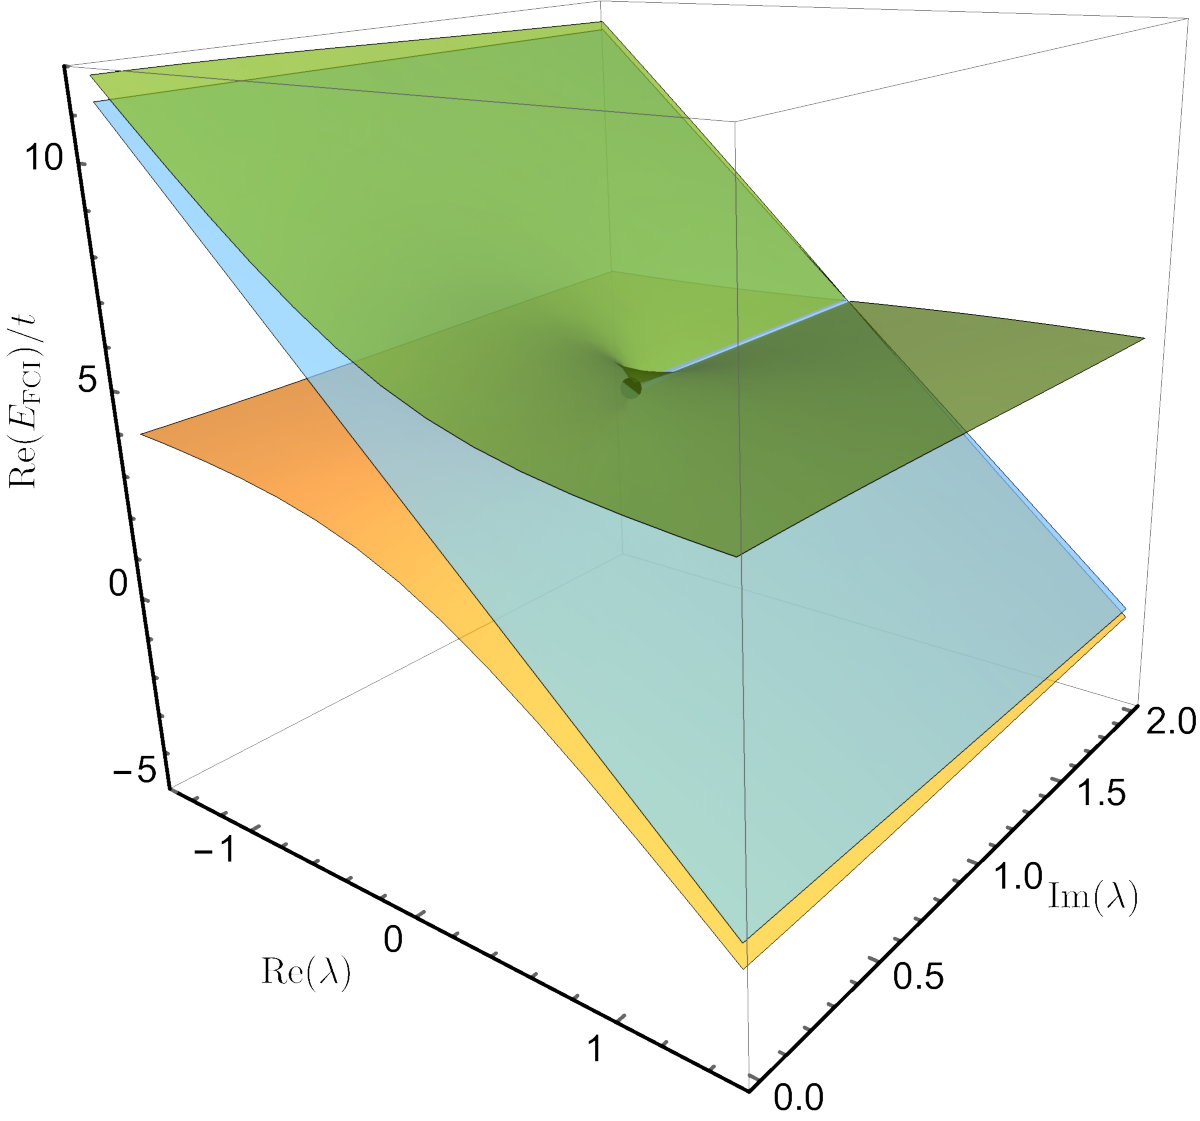
\includegraphics[height=0.75\textwidth]{fig2c}	
		\subcaption{\label{subfig:RMP_4.5} $U/t = 4.5$}
    \end{subfigure}
	\caption{
	Convergence of the RMP series as a function of the perturbation order $n$ for the Hubbard dimer at $U/t = 3.5$ (where $r_c > 1$) and $4.5$ (where $r_c < 1$).
	The Riemann surfaces associated with the exact energies of the RMP Hamiltonian \eqref{eq:H_RMP} are also represented for these two values of $U/t$ as functions of $\lambda$. 
	\label{fig:RMP}}
\end{figure*}

The behaviour of the UMP series is more subtle \hugh{than the RMP series as spin-contamination in the wave function
must be considered, introducing additional coupling between electronic states.
Using the ground-state UHF reference orbitals in the Hubbard dimer yields the UMP Hamiltonian}
\begin{widetext}
\begin{equation}
\label{eq:H_UMP}
\bH_\text{UMP}\hugh{\qty(\lambda)} = 
	\begin{pmatrix}
		-2t^2 \lambda/U	&	0									&	0									&	2t^2 \lambda/U		\\
		0				&	U - 2t^2 \lambda/U 					&	2t^2\lambda/U						&	2t \sqrt{U^2 - (2t)^2} \lambda/U	\\
		0				&	2t^2\lambda/U						&	U - 2t^2 \lambda/U 					&	-2t \sqrt{U^2 - (2t)^2} \lambda/U	\\
		2t^2 \lambda/U	&	2t \sqrt{U^2 - (2t)^2} \lambda/U 	&	-2t \sqrt{U^2 - (2t)^2} \lambda/U	&	2U(1-\lambda) + 6t^2\lambda/U		\\
	\end{pmatrix}.
\end{equation}
\end{widetext}
While there is a closed-form expression for the ground-state energy, it is cumbersome and we eschew reporting it.
Instead, the radius of convergence of the UMP series can obtained numerically as a function of $U/t$, as shown
in Fig.~\ref{fig:RadConv}.
\hugh{These numerical values reveal that the UMP ground state series has $\rc > 1$ for all $U/t$ and must always converge.
However, in the strong correlation limit (large $U$), this radius of convergence tends to unity, indicating that
the corresponding UMP series will become increasingly slow.
Furthermore, the doubly-excited state using the ground-state UHF orbitals has $\rc < 1$ for almost any value 
of $U/t$, reaching the limit value of $1/2$ for $U/t \rightarrow \infty$, and excited-state UMP series will always diverge.}
 
%%%%%%%%%%%%%%%%%%%%%%%%%%%%%
% RADIUS OF CONVERGENCE PLOTS
%%%%%%%%%%%%%%%%%%%%%%%%%%%%%
\begin{figure}
	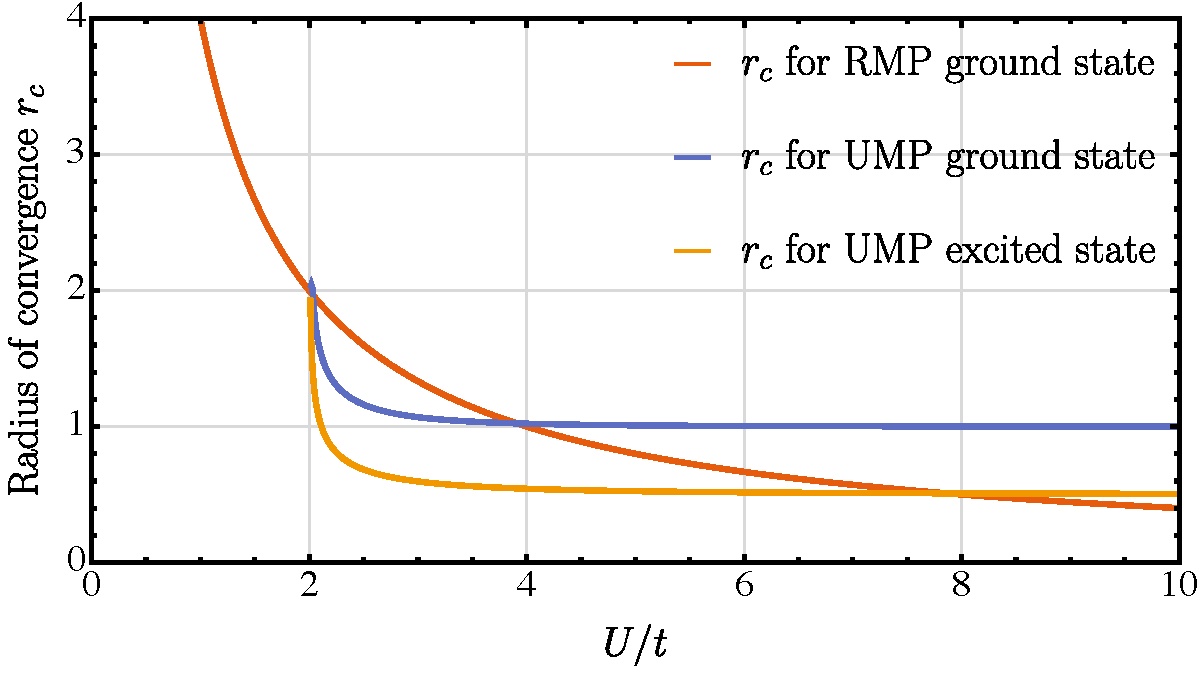
\includegraphics[width=\linewidth]{RadConv}
	\caption{
	Radius of convergence $r_c$ for the RMP ground state (red), the UMP ground state (blue), and the UMP excited state (orange) 
    series as functions of the ratio $U/t$.
	\label{fig:RadConv}}
\end{figure}
%%%%%%%%%%%%%%%%%%%%%%%%%%%%%
 
% DISCUSSION OF UMP RIEMANN SURFACES
The convergence of the UMP as a function of the ratio $U/t$ is shown in Fig.~\ref{subfig:UMP_cvg} for two specific values: the first ($U = 3t$) is well within the RMP convergence region, while the second ($U = 7t$) falls outside.
Note that in the case of UMP, there are now two pairs of EPs as the open-shell singlet now couples strongly with both the ground and doubly-excited states.
This has the clear tendency to move away from the origin the EP dictating the convergence of the ground-state energy, while deteriorating the convergence properties of the excited-state energy.
For $U = 3t$ (see Fig.~\ref{subfig:UMP_3}), the ground-state energy is remarkably flat since the UHF energy is already a pretty good estimate of the exact energy thanks to the symmetry-breaking process.
Most of the UMP expansion is actually correcting the spin-contamination in the wave function.
For $U = 7t$ (see Fig.~\ref{subfig:UMP_7}), we are well towards the strong correlation regime, where we see that the UMP series is slowly convergent while RMP diverges.
We see a single EP on the ground-state surface which falls just outside (maybe on?) the radius of convergence. 
An EP this close to the radius of convergence gives an increasingly slow convergence of the UMP series, but it will converge eventually as observed in Fig.~\ref{subfig:UMP_cvg}.
%On the other hand, there is an EP on the excited energy surface that is well within the radius of convergence.
%We can therefore say that the use of a symmetry-broken UHF wave function can retain a convergent ground-state perturbation series
%at the expense of a divergent excited-state perturbation series. (Note: the orbitals are not optimised for excited-state here).
%In contrast, the RMP expansion was always convergent for the open-shell excited state (which was a single CSF) while
%the radius of convergence for the doubly-excited state was identical to the ground-state as this was the only exceptional point.

%%% FIG 3 %%%
\begin{figure*}
	\begin{subfigure}{0.32\textwidth}
	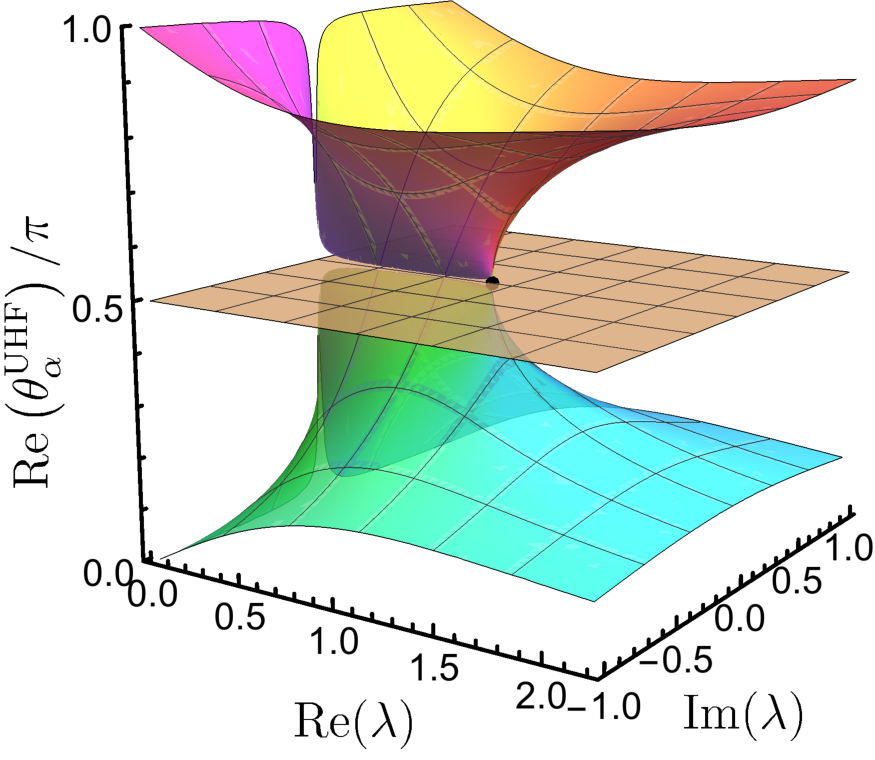
\includegraphics[height=0.75\textwidth]{fig3a}	
		\subcaption{\label{subfig:UMP_3} $U/t = 3$}
    \end{subfigure}
    %
    \begin{subfigure}{0.32\textwidth}
	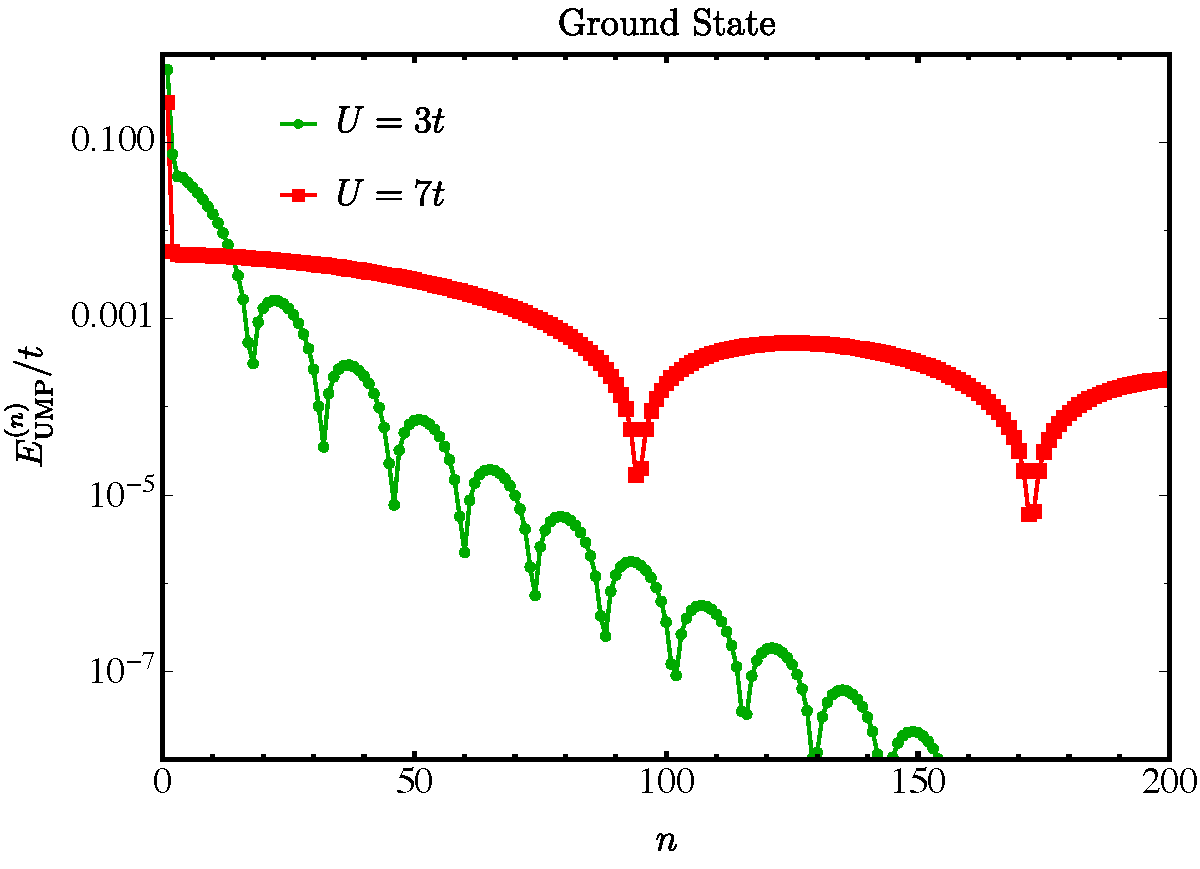
\includegraphics[height=0.75\textwidth]{fig3b}
		\subcaption{\label{subfig:UMP_cvg}}
    \end{subfigure}
    %
    \begin{subfigure}{0.32\textwidth}
	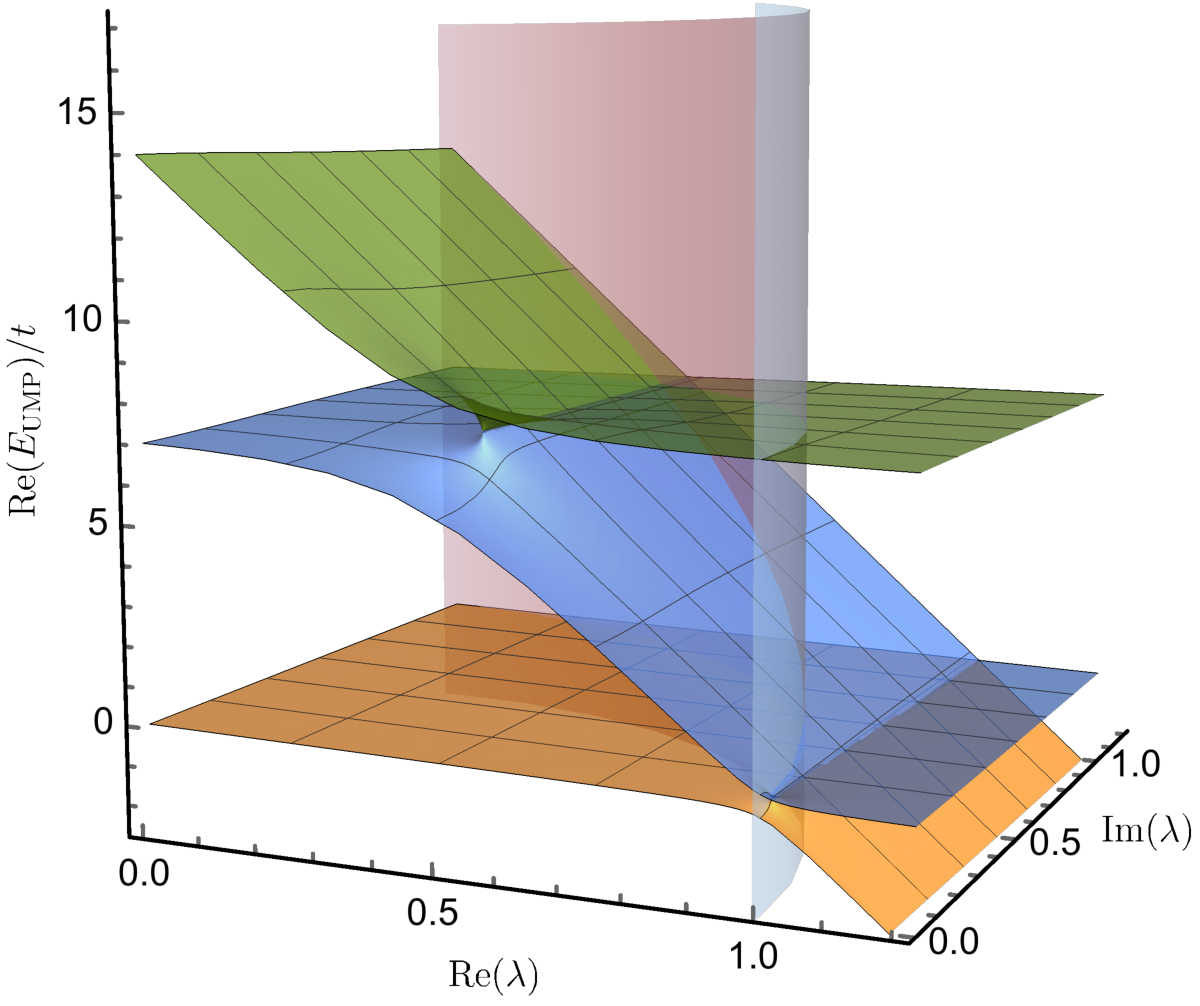
\includegraphics[height=0.75\textwidth]{fig3c}	
		\subcaption{\label{subfig:UMP_7} $U/t = 7$}
    \end{subfigure}	\caption{
	Convergence of the UMP series as a function of the perturbation order $n$ for the Hubbard dimer at $U/t = 3$ and $7$.
	The Riemann surfaces associated with the exact energies of the UMP Hamiltonian \eqref{eq:H_UMP} are also represented for these two values of $U/t$ as functions of $\lambda$.
	\label{fig:UMP}}
\end{figure*}

\hugh{(\textbf{HGAB}: Lets keep all the MP discussion together and add this note here)}
Obviously, although practically convenient for electronic structure calculations, the MP partitioning is not the only possibility, and alternative partitioning have been proposed in the literature:
i) the Epstein-Nesbet (EN) partitioning which consists in taking the diagonal elements of $\hH$ as the zeroth-order Hamiltonian. \cite{Nesbet_1955,Epstein_1926} 
Hence, the off-diagonal elements of $\hH$ are the perturbation operator,
ii) the weak correlation partitioning in which the one-electron part is consider as the unperturbed Hamiltonian $\hH^{(0)}$ and the two-electron part is the perturbation operator $\hV$, and 
iii) the strong coupling partitioning where the two operators are inverted compared to the weak correlation partitioning. \cite{Seidl_2018}

%%%%%%%%%%%%%%%%%%%%%%%%%%%%%%
\section{Historical overview}
%%%%%%%%%%%%%%%%%%%%%%%%%%%%%%

%=====================================================%
\subsection{Behavior of the M{\o}ller-Plesset series}
%=====================================================%

When one relies on MP perturbation theory (and more generally on any perturbative partitioning), it would be reasonable to ask for a systematic improvement of the energy with respect to the perturbative order, \ie, one would expect that the more terms of the perturbative series one can compute, the closer the result from the exact energy.
%In other words, each time a higher-order term is computed, one would like to obtained an overall result closer to the exact energy. 
In other words, one would like a monotonic convergence of the MP series. Assuming this, the only limiting process to get the exact correlation energy (in a finite basis set) would be our ability to compute the terms of this perturbation series.
Unfortunately this is not as easy as one might think because i) the terms of the perturbative series become rapidly computationally cumbersome, and ii) erratic behavior of the perturbative coefficients are not uncommon. For example, in the late 80's, Gill and Radom reported deceptive and slow convergences in stretched systems \cite{Gill_1986, Gill_1988} (see also Refs.~\onlinecite{Handy_1985, Lepetit_1988}). 
In Ref.~\onlinecite{Gill_1986}, the authors showed that the RMP series is convergent, yet oscillatory which is far from being convenient if one is only able to compute the first few terms of the expansion (for example here RMP5 is worse than RMP4). 
On the other hand, the UMP series is monotonically convergent (except for the first few orders) but very slowly. 
Thus, one cannot practically use it for systems where only the first terms can be computed.

When a bond is stretched, in most cases the exact wave function becomes more and more of multi-reference nature. 
Yet the HF wave function is restricted to be a single Slater determinant.
It is then inappropriate to model (even qualitatively) stretched systems. Nevertheless, the HF wave function can undergo symmetry breaking to lower its energy by sacrificing one of the symmetry of the exact wave function in the process (see for example the case of \ce{H2} in Ref.~\onlinecite{SzaboBook}). 
One could then potentially claim that the RMP series exhibits deceptive convergence properties as the RHF Slater determinant is a poor approximation of the exact wave function for stretched system. However, even in the unrestricted formalism which clearly represents a better description of a stretched system, the UMP series does not have the smooth and rapidly convergent behavior that one would wish for. 

In the unrestricted framework the singlet ground state wave function is allowed to mix with triplet wave functions, leading to the so-called spin contamination issue. Gill \textit{et al.}~highlighted the link between slow convergence of the UMP series and spin contamination for \ce{H2} in a minimal basis. \cite{Gill_1988}
Handy and coworkers reported the same behavior of the series (oscillatory and slowly monotonically convergent) in stretched \ce{H2O} and \ce{NH2}. \cite{Handy_1985} Lepetit \textit{et al.}~analyzed the difference between the MP and EN partitioning for the UHF reference. \cite{Lepetit_1988} 
They concluded that the slow convergence is due to the coupling of the singly- and doubly-excited configurations. 
Cremer and He analyzed 29 atomic and molecular systems at the FCI level \cite{Cremer_1996} and grouped them in two classes: i) the \textit{class A} systems where one observes a monotonic convergence to the FCI energy, and ii) the \textit{class B} systems for which convergence is erratic after initial oscillations. Their system set contains stretched molecules as well as molecules at their equilibrium geometry for various basis sets. They highlighted that \cite{Cremer_1996}
\textit{``Class A systems are characterized by electronic structures with well-separated electron pairs while class B systems are characterized by electronic structures with electron clustering in one or more regions.''}
Moreover, they analyzed the contribution of the triple (T) excitations to the MP4, MP5 and MP6 energies next to the single, double and quadruple (SDQ) excitations contribution.
They showed that class A systems have very little contribution from the triple excitations and that most of the correlation energy is due to pair correlation. On the other hand, class B systems have an important contribution from the triple excitations which alternates in sign resulting in an oscillation of the total correlation energy.
This observation on the contribution to the MPn energy corroborates the electronic structure discussed above.
As one can only compute the first terms of the MP series, a smart way of getting more accurate results is to use extrapolation formula, \ie, estimating the limit of the series with only few terms. 
Cremer and He proved that using specific extrapolation formulas of the MP series for class A and class B systems improves the precision of the results compared to the formula used without resorting to classes. The mean absolute deviation taking the FCI correlation energies as reference is $0.3$ millihartree with the class-specific formula whereas the deviation increases to 12 millihartree using the general formula.  
Even if there were still shaded areas in their analysis and that their classification was incomplete, the work of Cremer and He clearly evidenced that understanding the origin of the different modes of convergence could potentially lead to a more rationalized use of MP perturbation theory and, hence, to more accurate correlation energy estimates.

Recently, Mih\'alka \textit{et al.} studied the partitioning effect on the convergence properties of Rayleigh-Schr\"odinger perturbation theory by considering the MP and the EN partitioning as well as an alternative partitioning. \cite{Mihalka_2017a} 
Taking as an example (in particular) the water molecule at equilibrium and at stretched geometries, they could estimate the radius of the convergence via a quadratic Pad\'e approximant and convert divergent perturbation expansions to convergent ones in some cases thanks to a judicious choice of the level shift parameter.
In a subsequent study by the same group, \cite{Mihalka_2017b} they use analytic continuation techniques to resum divergent MP series taking again as an example the water molecule in a stretched geometry.
In a nutshell, their idea consists in calculating the energy of the system for several values of $\lambda$ for which the MP series is rapidly convergent, and to extrapolate the final energy to the physical system at $\lambda = 1$ via a polynomial- or Pad\'e-based fit. 
However, the choice of the functional form of the fit remains a subtle task.
This technique was first generalized by using complex scaling parameters and applying analytic continuation by solving the Laplace equation, \cite{Surjan_2018} and then further improved thanks to Cauchy's integral formula \cite{Mihalka_2019}
\begin{equation}
	\label{eq:Cauchy}
	\frac{1}{2\pi i} \oint_{\gamma} \frac{E(z)}{z - a} = E(a),
\end{equation}
which states that the value of the energy can be computed at $z=a$ inside the contour $\gamma$ only by the knowledge of its values on the same contour.
Their method consists in refining self-consistently the values of $E(z)$ computed on a contour going through the physical point at $z = 1$ and encloses points of the ``trusted'' region (where the MP series is convergent). The shape of this contour is arbitrary but no singularities are allowed inside the contour to ensure $E(z)$ is analytic. 
When the values of $E(z)$ on the so-called contour are converged, Cauchy's integrals formula \eqref{eq:Cauchy} is invoked to compute the values at $E(z=1)$ which corresponds to the final estimate of the FCI energy.
The authors illustrate this protocol on the dissociation curve of \ce{LiH} and the stretched water molecule showing encouraging results. \cite{Mihalka_2019} 

%==========================================%
\subsection{Insights from a two-state model}
%==========================================%

In the late 90's, Olsen \textit{et al.}~discovered an even more preoccupying behavior of the MP series. \cite{Olsen_1996} They showed that the series could be divergent even in systems that they considered as well understood like \ce{Ne} and \ce{HF}. \cite{Olsen_1996, Christiansen_1996} Cremer and He had already studied these two systems and classified them as \textit{class B} systems. However, the analysis of Olsen and coworkers was performed in larger basis sets containing diffuse functions. In these basis sets, they found that the series become divergent at (very) high order.

The discovery of this divergent behavior is worrying as in order to get meaningful and accurate energies, calculations must be performed in large basis sets (as close as possible from the complete basis set limit). Including diffuse functions is particularly important in the case of anions and/or Rydberg excited states where the wave function is much more diffuse than the ground-state one. As a consequence, they investigated further the causes of these divergences as well as the reasons of the different types of convergence. To do so, they analyzed the relation between the dominant singularity (\ie, the closest singularity to the origin) and the convergence behavior of the series. \cite{Olsen_2000} Their analysis is based on Darboux's theorem: 
\begin{quote}
	\textit{``In the limit of large order, the series coefficients become equivalent to the Taylor series coefficients of the singularity closest to the origin. Following the result of this theorem, the convergence patterns of the MP series can be explained by looking at the dominant singularity.''}
\end{quote}

A singularity in the unit circle is designated as an intruder state, more precisely as a front-door (respectively back-door) intruder state if the real part of the singularity is positive (respectively negative). Their method consists in performing a scan of the real axis to detect the avoided crossing responsible for the pair of dominant singularities. Then, by modeling this avoided crossing via a two-state Hamiltonian one can get an approximation of the dominant conjugate pair of singularities by finding the EPs of the following $2\times2$ matrix
\begin{equation}
	\underbrace{\mqty(\alpha & \delta \\ \delta & \beta)}_{\bH} = \underbrace{\mqty(\alpha & 0 \\ 0 & \beta + \gamma )}_{\bH^{(0)}} + \underbrace{\mqty( 0 & \delta \\ \delta & - \gamma)}_{\bV},
\end{equation}
where the diagonal matrix is the unperturbed Hamiltonian matrix $\bH^{(0)}$ and the second matrix in the right-hand-side $\bV$ is the perturbation.

They first studied molecules with low-lying doubly-excited states of the same spatial and spin symmetry.
The exact wave function has a non-negligible contribution from the doubly-excited states, so these low-lying excited states were good candidates for being intruder states. \titou{For \ce{CH_2} in a large basis set, the series is convergent up to the 50th order. They showed that the dominant singularity lies outside the unit circle but close to it causing the slow convergence.}

Then they demonstrated that the divergence for \ce{Ne} is due to a back-door intruder state. When the basis set is augmented with diffuse functions, the ground state undergo sharp avoided crossings with highly diffuse excited states leading to a back-door intruder state. They used their two-state model on this avoided crossings and the model was actually predicting the divergence of the series. 
%They concluded that the divergence of the series was due to the interaction with a highly diffuse excited state. 

Moreover they proved that the extrapolation formulas of Cremer and He \cite{Cremer_1996} cannot be used for all systems, and that these formulas were not mathematically motivated when looking at the singularity causing the divergence. 
For example, the hydrogen fluoride molecule contains both back-door intruder states and low-lying doubly-excited states which results in alternated terms up to 10th order. 
For higher orders, the series is monotonically convergent. This surprising behavior is due to the fact that two pairs of singularities are approximately at the same distance from the origin.


In Ref.~\onlinecite{Olsen_2019}, the simple two-state model proposed by Olsen \textit{et al.} is generalized to a non-symmetric Hamiltonian 
\begin{equation}
	\underbrace{\mqty(\alpha & \delta_1 \\ \delta_2 & \beta)}_{\bH} = \underbrace{\mqty(\alpha & 0 \\ 0 & \beta + \gamma )}_{\bH^{(0)}} + \underbrace{\mqty( 0 & \delta_2 \\ \delta_1 & - \gamma)}_{\bV}.
\end{equation}
allowing an analysis of various choice of perturbation (not only the MP partioning) such as coupled cluster perturbation expansions \cite{Pawlowski_2019a,Pawlowski_2019b,Pawlowski_2019c,Pawlowski_2019d,Pawlowski_2019e} and other non-Hermitian perturbation methods.
It is worth noting that only cases where $\text{sgn}(\delta_1) = - \text{sgn}(\delta_2)$ leads to new forms of perturbation expansions.
Interestingly, they showed that the convergence pattern of a given perturbation method can be characterized by its archetype which defines the overall ``shape'' of the energy convergence. These so-called archetypes can be subdivided in five classes for Hermitian Hamiltonians (zigzag, interspersed zigzag, triadic, ripples, and geometric), while two additional archetypes (zigzag-geometric and convex-geometric) are observed in non-Hermitian Hamiltonians.
Importantly, they observed that the geometric archetype is the most common for MP expansions but that the ripples archetype sometimes occurs. \cite{Handy_1985,Lepetit_1988,Leininger_2000}
Other features characterizing the convergence behavior of a perturbation method are its rate of convergence, its length of recurring period, and its sign pattern;
the three remaining archetypes seem to be rarely observed in MP perturbation theory.
However, in the non-Hermitian setting of coupled cluster perturbation theory, \cite{Pawlowski_2019a,Pawlowski_2019b,Pawlowski_2019c,Pawlowski_2019d,Pawlowski_2019e} on can encounter interspersed zigzag, triadic, ripple, geometric, and zigzag-geometric archetypes.
One of main take-home messages of Olsen's study is that the primary critical point defines the high-order convergence, irrespective of whether this point is inside or outside the complex unit circle. \cite{Handy_1985,Olsen_2000}

%=======================================
\subsection{The singularity structure}
%=======================================
In the 2000's, Sergeev and Goodson \cite{Sergeev_2005, Sergeev_2006} analyzed this problem from a more mathematical point of view by looking at the whole singularity structure where Olsen and collaborators were trying to find the dominant singularity causing the divergence. They regrouped singularities in two classes: i) $\alpha$ singularities which have ``large'' imaginary parts, and ii) $\beta$ singularities which have very small imaginary parts. Singularities of type $\alpha$ are related to large avoided crossing between the ground and low-lying excited states, whereas $\beta$ singularities come from a sharp avoided crossing between the ground state and a highly diffuse state. They succeeded to explain the divergence of the series caused by $\beta$ singularities following previous work of Stillinger. \cite{Stillinger_2000}

To understand the convergence properties of the perturbation series at $\lambda=1$, one must look at the whole complex plane, in particular, for negative (\ie, real) values of $\lambda$. If $\lambda$ is negative, the Coulomb interaction becomes attractive but the mean field (which has been computed at $\lambda = 1$) remains repulsive as it is proportional to $(1-\lambda)$:

\begin{multline}
\label{eq:HamiltonianStillinger}
    \hH(\lambda) = 
    \sum_{i}^{n} \Bigg[ 
    \overbrace{-\frac{1}{2}\grad_i^2 
    - \sum_{A}^{N} \frac{Z_A}{\abs{\vb{r}_i-\vb{R}_A}}}^{\text{independent of $\lambda$}}
    \\
    + \underbrace{(1-\lambda)v^{\text{HF}}(\vb{x}_i)}_{\text{repulsive for $\lambda < 1$}}
    + \underbrace{\lambda\sum_{i<j}^{n}\frac{1}{|\vb{r}_i-\vb{r}_j|}}_{\text{attractive for $\lambda < 0$}}
    \Bigg].
\end{multline}

The major difference between these two terms is that the repulsive mean field is localized around the nuclei whereas the interelectronic interaction persist away from the nuclei. If $\lambda$ becomes more and more negative the mean field becomes more and more repulsive so there exists a critical (negative) value of $\lambda$, $\lambda_\text{c}$, for which the Coulombic field created by the nuclei cannot bind the electrons anymore because of the $\lambda$-independent nature of the electron-nucleus attraction. For $\lambda = \lambda_c$, the electrons dissociate from the nuclei and form a bound cluster which is infinitely separated from the nuclei. According to Baker, \cite{Baker_1971} this value is a critical point of the system and, by analogy with thermodynamics, the energy $E(\lambda)$ exhibits a singularity at $\lambda_\text{c}$. At this point the system undergo a phase transition and a symmetry breaking. 
Beyond $\lambda_c$ there is a continuum of eigenstates thanks to which the electrons dissociated from the nuclei.

This reasoning is done on the exact Hamiltonian and energy, \ie, the Hamiltonian in the complete Hilbert space, this is the exact energy which exhibits this singularity on the negative real axis. However, in a finite basis set which does not span the complete Hilbert space, one can prove that, for a Hermitian Hamiltonian, the singularities of $E(\lambda)$ occurs in complex conjugate pairs with non-zero imaginary parts. Sergeev and Goodson proved, \cite{Sergeev_2005} as predicted by Stillinger, \cite{Stillinger_2000} that in a finite basis set the critical point on the real axis is modeled by a cluster of sharp avoided crossings with diffuse functions, equivalently by a cluster of $\beta$ singularities in the negative half plane. This explains that Olsen \textit{et al.}, because they used a simple $2\times2$ model, only observed the first singularity of this cluster of singularities causing the divergence. \cite{Olsen_2000}

Finally, it was shown that $\beta$ singularities are very sensitive to changes in the basis set but not to the stretching of the system. On the contrary, $\alpha$ singularities are relatively insensitive to the basis sets but very sensitive to bond stretching. 
According to Goodson, \cite{Goodson_2004} the singularity structure of stretched molecules is difficult because there is more than one significant singularity. 
This is consistent with the observation of Olsen and coworkers \cite{Olsen_2000} on the \ce{HF} molecule at equilibrium geometry and stretched geometry. 
To the best of our knowledge, the effect of bond stretching on singularities, its link with spin contamination and symmetry breaking of the wave function has not been as well understood as the ionization phenomenon and its link with diffuse functions.  

%====================================================
\subsection{The physics of quantum phase transitions}
%====================================================

In the previous section, we saw that a careful analysis of the structure of the Hamiltonian allows us to predict the existence of a critical point. In a finite basis set this critical point is model by a cluster of $\beta$ singularities. It is now well known that this phenomenon is a special case of a more general phenomenon. Indeed, theoretical physicists proved that EPs close to the real axis are connected to \textit{quantum phase transitions} (QPTs). \cite{Heiss_1988,Heiss_2002,Cejnar_2005, Cejnar_2007, Cejnar_2009, Borisov_2015, Sindelka_2017} In quantum mechanics, the Hamiltonian is almost always dependent of, at least, one parameter. In some cases the variation of a parameter can lead to abrupt changes at a critical point. These QPTs exist both for ground and excited states as shown by Cejnar and coworkers. \cite{Cejnar_2009, Sachdev_2011, Cejnar_2015, Cejnar_2016, Caprio_2008, Macek_2019} A ground-state QPT is characterized by the derivatives of the ground-state energy with respect to a non-thermal control parameter. \cite{Cejnar_2009, Sachdev_2011} The transition is called discontinuous and of first order if the first derivative is discontinuous at the critical parameter value. Otherwise, it is called continuous and of $m$th order if the $m$th derivative is discontinuous. A QPT can also be identify by the discontinuity of an appropriate order parameter (or one of its derivatives). 

The presence of an EP close to the real axis is characteristic of a sharp avoided crossing. Yet, at such an avoided crossing, eigenstates change abruptly. Although it is now well understood that EPs are closely related to QPTs, the link between the type of QPT (ground state or excited state, first or higher order) and EPs still need to be clarified. One of the major obstacles that one faces in order to achieve this resides in the ability to compute the distribution of EPs. The numerical assignment of an EP to two energies on the real axis is very difficult in large dimensions. Hence, the design of specific methods are required to get information on the location of EPs. Following this idea, Cejnar \textit{et al.}~developed a method based on a Coulomb analogy giving access to the density of EP close to the real axis. \cite{Cejnar_2005, Cejnar_2007} More recently Stransky and coworkers proved that the distribution of EPs is characteristic on the order of the QPT. \cite{Stransky_2018} In the thermodynamic limit, some of the EPs converge towards a critical point $\lambda_\text{c}$ on the real axis. They showed that, within the interacting boson model, \cite{Lipkin_1965} EPs associated to first- and second-order QPT behave differently when the number of particles increases. The position of these singularities converge towards the critical point on the real axis at different rates (exponentially and algebraically for the first and second orders, respectively) with respect to the number of particles.

Moreover, Cejnar \textit{et al.}~studied the so-called shape-phase transitions of the IBM model from the QPT's point of view \cite{Cejnar_2000, Cejnar_2003, Cejnar_2007a, Cejnar_2009}. The phase of the ensemble of $s$ and $d$ bosons is characterized by a dynamical symmetry. When a parameter is continously modified the dynamical symmetry of the system can change at a critical value of this parameter, leading to a deformed phase. They showed that at this critical value of the parameter, the system undergoes a QPT. For example, without interaction the ground state is the spherical phase (a condensate of s bosons) and when the interaction increases it leads to a deformed phase constituted of a mixture of s and d bosons states. In particular, we see that the transition from the spherical phase to the axially symmetric one is analog to the symmetry breaking of the wavefunction of the hydrogen molecule when the bond is stretched \cite{SzaboBook}.
It seems like our understanding of the physics of spatial and/or spin symmetry breaking in HF theory can be enlightened by QPT theory. Indeed, the second derivative of the HF ground-state energy is discontinuous at the point of spin symmetry-breaking which means that the system undergo a second-order QPT. Moreover, the $\beta$ singularities introduced by Sergeev and coworkers to describe the EPs modeling the formation of a bound cluster of electrons are actually a more general class of singularities. The EPs close to the real axis (the so-called $\beta$ singularities) are connected to QPT because they result from a sharp avoided crossings at which the eigenstates change quickly. However, the $\alpha$ singularities arise from large avoided crossings. Thus, they cannot be connected to QPT. The avoided crossings generating $\alpha$ singularities generally involve the ground state and low-lying doubly-excited states. Those excited states have a non-negligible contribution to the exact FCI solution because they have (usually) the same spatial and spin symmetry as the ground state. We believe that $\alpha$ singularities are connected to states with non-negligible contribution in the CI expansion thus to the dynamical part of the correlation energy, while $\beta$ singularities are linked to symmetry breaking and phase transitions of the wave function, \ie, to the multi-reference nature of the wave function thus to the static part of the correlation energy.


%%============================================================%
%\section{The spherium model}
%\label{sec:spherium}
%%============================================================%
%
%Simple systems that are analytically solvable (or at least quasi-exactly solvable, \ie, models for which it is possible to obtain a finite portion of the exact solutions of the Schr{\"o}dinger equation \cite{Ushveridze_1994}) are of great importance in theoretical chemistry. 
%These systems are very useful to perform benchmark studies in order to test new methods as the mathematics are easier than in realistic systems (such as molecules or solids) but retain much of the key physics. 
%To investigate the physics of EPs we consider one such system named \textit{spherium}. 
%It consists of two electrons confined to the surface of a sphere interacting through the long-range Coulomb potential. \cite{Thompson_2005, Seidl_2007, Loos_2009b} 
%Thus, the Hamiltonian is
%\begin{equation}
%	\hH = -\frac{\grad_1^2 + \grad_2^2}{2} + \frac{1}{r_{12}},
%\end{equation}
%or
%\begin{equation} \label{eq:H-sph-omega}
%	\hH = -\frac{1}{R^2} \qty( \pdv[2]{}{\omega} + \cot \omega \pdv{}{\omega}) + \frac{1}{R \sqrt{2 - 2 \cos \omega}},
%\end{equation}
%in term of the interelectronic angle $\omega$.
%The Laplace operators are the kinetic operators for each electron and $r_{12}^{-1} = \abs{\vb{r}_1 - \vb{r}_2}^{-1}$ is the Coulomb operator. 
%Note that, as readily seen by the definition of the interelectronic distance $r_{12}$, the electrons interact through the sphere.
%The radius of the sphere $R$ dictates the correlation regime. \cite{Loos_2009}
%In the weak correlation regime (\ie, small $R$), the kinetic energy (which scales as $R^{-2}$) dominates and the electrons are delocalized over the sphere.
%For large $R$ (or strong correlation regime), the electron repulsion term (which scales as $R^{-1}$) drives the physics and the electrons localize on opposite side of the sphere to minimize their Coulomb repulsion. 
%This phenomenon is sometimes referred to as a Wigner crystallization. \cite{Wigner_1934}
%
%We will use this model in order to rationalize the effects of the parameters that may influence the physics of EPs:
%i) Partitioning of the Hamiltonian and the actual zeroth-order reference: weak correlation reference (RHF or UHF references, MP or EN partitioning), or strongly correlated reference.
%ii) Basis set: minimal basis or infinite (\ie, complete) basis.
%iii) Radius of the sphere that ultimately dictates the correlation regime.
%
%In the RHF formalism, the two electrons are restricted to ``live'' in the same spatial orbital.
%The spatial part of the RHF wave function is then
%\begin{equation}\label{eq:RHF_WF}
%	\Psi_{\text{RHF}}(\theta_1,\theta_2) = Y_0(\theta_1) Y_0(\theta_2),
%\end{equation}
%where $\theta_i$ is the polar angle of the $i$th electron and $Y_{\ell}(\theta)$ is a zonal spherical harmonic. 
%Because $Y_0(\theta) = 1/\sqrt{4\pi}$, it is clear that the RHF wave function yields a uniform one-electron density.
%
%The RHF wave function cannot model properly the physics of the system at large $R$ because the spatial orbitals are restricted to be the same, and, \textit{a fortiori}, it cannot represent two electrons on opposite side of the sphere. 
%Within the UHF formalism, there is a critical value of $R$, called Coulson-Fischer point, \cite{Coulson_1949} at which a UHF solution appears and is lower in energy than the RHF one.
%The UHF solution has broken symmetry because the two electrons tends to localize on opposite sides of the sphere. 
%The spatial part of the UHF wave function is defined as
%\begin{equation}\label{eq:UHF_WF}
%	\Psi_{\text{UHF}}(\theta_1,\theta_2)=\phi_\alpha(\theta_1)\phi_\beta(\theta_2),
%\end{equation}
%where $\phi_\sigma(\theta)$ is the spatial orbital associated with the spin-$\sigma$ electrons ($\sigma = \alpha$ for spin-up electrons and $\sigma = \beta$ for spin-down electrons).
%These one-electron orbitals are expanded in the basis of zonal spherical harmonics
%\begin{equation}
%	\phi_\sigma(\theta)=\sum_{\ell=0}^{\infty}C_{\sigma,\ell}Y_{\ell}(\theta).
%\end{equation}
%It is possible to obtain the formula for the HF energy in this basis set: \cite{Loos_2009}
%\begin{equation}
%	E_{\text{HF}} = T_{\text{HF}} + V_{\text{HF}},
%\label{eq:EHF}
%\end{equation}
%where the kinetic and potential energies are, respectively,
%\begin{align}
%	T_{\text{HF}} & = \frac{1}{R^2} \sum_{\sigma=\alpha,\beta} \sum_{\ell=0}^{\infty} C_{\sigma,\ell}^2 \, \ell(\ell+1),
%	&
%	V_{\text{HF}} & = \frac{1}{R} \sum_{L=0}^{\infty}
%	v^\alpha_{L} v^\beta_{L},
%\end{align}
%and
%\begin{equation}
%	v^\sigma_{L} 
%	=  \sum_{\ell_1,\ell_2} \sqrt{(2\ell_1+1)(2\ell_2+1)} C_{\sigma,\ell_1}C_{\sigma,\ell_2}
%	\begin{pmatrix}
%		\ell_1 & L & \ell_2 
%		\\
%		0 & 0 & 0
%	\end{pmatrix}^2 
%\end{equation}
%is expressed in terms of the Wigner 3j-symbols. \cite{AngularBook}
%
%The general method is to use a self-consistent field procedure as described in Ref.~\onlinecite{SzaboBook} to get the coefficients of the HF wave function corresponding to stationary solutions with respect to the coefficients $C_{\sigma,\ell}$, \ie,
%\begin{equation}
%	\pdv{E_{\text{HF}}}{C_{\sigma,\ell}} = 0.
%\end{equation}
%Here, we work in a minimal basis, composed of $Y_{0}$ and $Y_{1}$, or equivalently, a $s$ and $p_{z}$ orbital, to illustrate the difference between the RHF and UHF solutions. In this basis there is a shortcut to find the stationary solutions and ensure normalization of the orbitals. One can define the one-electron orbitals as
%\begin{equation}
%	\phi_\sigma(\theta)= \cos(\chi_\sigma)Y_{0}(\theta) + \sin(\chi_\sigma)Y_{1}(\theta),
%\end{equation}
%using a mixing angle $\chi_\sigma$ between the two basis functions for each spin manifold. 
%Hence, one has just to minimize/maximize the energy with respect to the two mixing angles $\chi_\alpha$ and $\chi_\beta$.
% 
%This process provides the three following solutions valid for all value of $R$, which are respectively a minimum, a maximum and a saddle point of the HF equations:
%i) the two electrons are in the $s$ orbital which is a RHF solution. This solution is associated with the energy $1/R$;
%ii) the two electrons are in the $p_{z}$ orbital which is a RHF solution. This solution is associated with the energy $2/R^{2}+ 29/(25R)$;
%iii) one electron is in the $s$ orbital and the other is in the $p_{z}$ orbital which is a UHF solution. This solution is associated with the energy $1/R^{2} + 1/R$.
%
%In addition, the minimization process gives also the well-known symmetry-broken UHF (sb-UHF) solution. In this case the Coulson-Fischer point associated to this solution is $R=3/2$. 
%For $R>3/2$, the sb-UHF solution is the global minimum of the HF equations and the RHF solution presented before is a local minimum. This solution corresponds to the configuration with the spin-up electron in an orbital on one side of the sphere and the spin-down electron in a miror-image orbital on the opposite side and the configuration the other way round. The electrons can be on opposite sides of the sphere because the choice of $p_{z}$ as a basis function induced a privileged axis on the sphere for the electrons. For $R>3/2$, this solution has the energy
%\begin{equation}\label{eq:EsbUHF}
%	E_{\text{sb-UHF}}=-\frac{75}{112R^3}+\frac{25}{28R^2}+\frac{59}{84R}.
%\end{equation}
%
%The exact solution for the ground state is a singlet. The spherical harmonics are eigenvectors of $\hS^2$ (the spin operator) and they are associated to different eigenvalues. 
%Yet, the symmetry-broken orbitals are linear combinations of $Y_0$ and $Y_1$. 
%Hence, the symmetry-broken orbitals are not eigenvectors of $\hS^2$. 
%However, this solution gives lower energies than the RHF one at large $R$, even if it does not have the exact spin symmetry. 
%In fact, at the Coulson-Fischer point, it becomes more effective to minimize the Coulomb repulsion than the kinetic energy in order to minimize the total energy. 
%Thus, within the HF approximation, the variational principle is allowed to break the spin symmetry because it yields a more effective minimization of the Coulomb repulsion. 
%This type of symmetry breaking is also called a spin-density wave in the physics community as the system ``oscillates'' between the two symmetry-broken configurations. \cite{GiulianiBook}
%
%There is also another symmetry-broken solution for $R>75/38$ but this one corresponds to a maximum of the HF equations. 
%This solution is associated with another type of symmetry breaking somewhat less known. 
%It corresponds to a configuration where both electrons are on the same side of the sphere, in the same spatial orbital. 
%This solution is called symmetry-broken RHF (sb-RHF). The reasoning is counter-intuitive because the electrons tends to maximize their energy. 
%The $sp_{z}$ orbital is symmetric with respect to the center of the sphere. 
%If the orbitals are symmetric, the maximum is when the two electrons are in the $p_{z}$ orbital because it maximizes the kinetic energy. 
%At the critical value of $R$, placing the two electrons in the same symmetry-broken orbital \ie, on the same side of the sphere gives a superior energy than the $p_{z}^2$ state. Adding a s orbital on one side of the $p_{z}$ orbital to form a symmetry-broken orbital reduce the kinetic energy but increase the repulsion energy as the two electrons are more localized on one side of the sphere. 
%It becomes more efficient to maximize the repulsion energy than the kinetic energy for $R>75/38$. 
%This configuration breaks the spatial symmetry of charge. 
%Hence this symmetry breaking is associated with a charge-density wave as the system oscillates between the situations where the two electrons are one side or the other. \cite{GiulianiBook}
%The energy associated with this sb-RHF solution reads
%\begin{equation}
%E_{\text{sb-RHF}}=\frac{75}{88R^3}+\frac{25}{22R^2}+\frac{91}{66R}.
%\end{equation}
%\begin{figure}
%    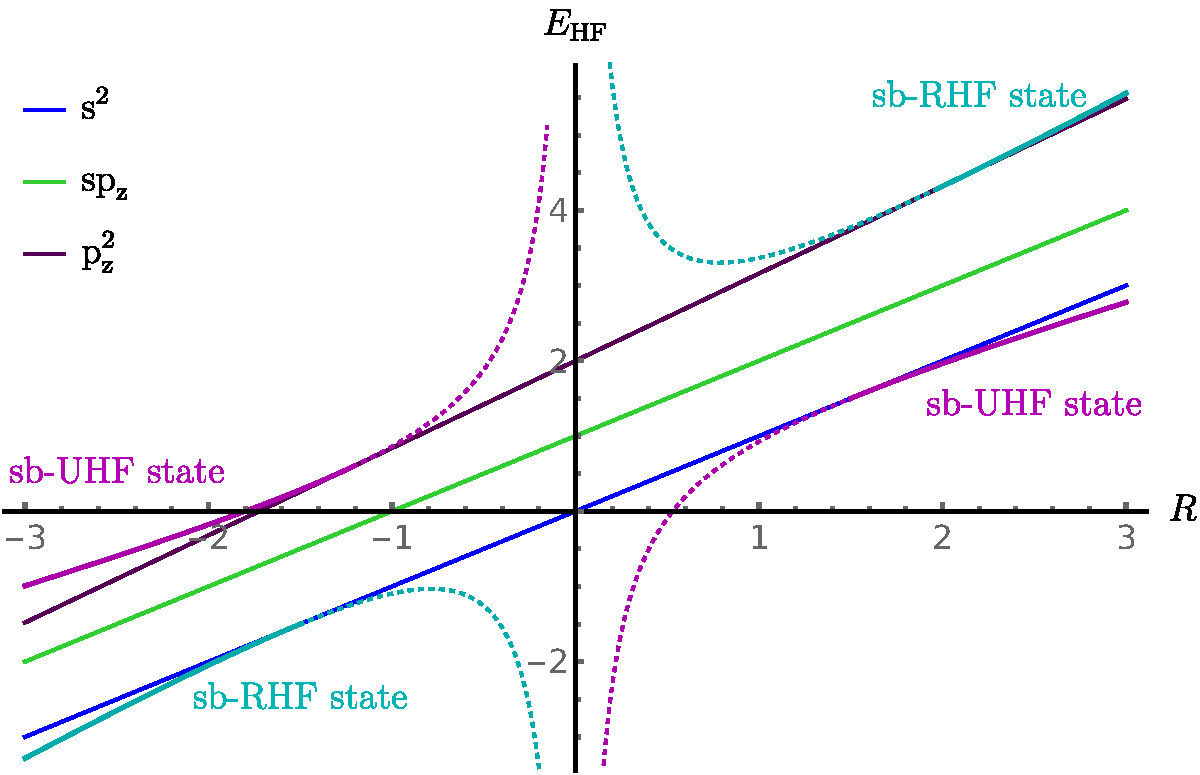
\includegraphics[width=\linewidth]{EsbHF.pdf}
%    \caption{Energies of the five solutions of the HF equations (multiplied by $R^2$). The dotted curves correspond to the analytic continuation of the symmetry-broken solutions.}
%    \label{fig:SpheriumNrj}
%\end{figure}
%
%We can also consider negative values of $R$, which corresponds to the situation where one of the electrons is replaced by a positron as readily seen in Eq.~\eqref{eq:H-sph-omega}. 
%For negative $R$ values, there are also a sb-RHF ($R<-3/2$) and a sb-UHF ($R<-75/38$) solution for negative values of $R$ (see Fig.~\ref{fig:SpheriumNrj}) but in this case the sb-RHF solution is a minimum and the sb-UHF is a maximum of the HF equations. 
%Indeed, the sb-RHF state minimizes the attraction energy by placing the electron and the positron on the same side of the sphere. 
%And the sb-UHF state maximizes the energy because the two attracting particles are on opposite sides of the sphere.
%
%In addition, we can also consider the symmetry-broken solutions beyond their respective Coulson-Fischer points by analytically continuing their respective energies leading to the so-called holomorphic solutions. \cite{Hiscock_2014, Burton_2019, Burton_2019a} All those energies are plotted in Fig.~\ref{fig:SpheriumNrj}. The dotted curves corresponds to the holomorphic domain of the energies.
%
%
%\section{Radius of convergence and exceptional points}
%
%\subsection{Evolution of the radius of convergence}
%
%In this subsection, we investigate how the partitioning of $\hH(\lambda)$ influence the radius of convergence of the perturbation series. Let us remind the reader that the radius of convergence is equal to the distance of the closest singularity to the origin of $E(\lambda)$. Hence, we have to determine the locations of the EPs to obtain information on the convergence properties of the perturbative series. To find them we solve simultaneously the following equations: \cite{Cejnar_2007}
%\begin{subequations}
%\begin{align}
%	\label{eq:PolChar}
%	\det[E\hI-\hH(\lambda)] & = 0,
%	\\ 
%	\label{eq:DPolChar}
%	\pdv{E}\det[E\hI-\hH(\lambda)] & = 0,
%\end{align}
%\end{subequations}
%where $\hI$ is the identity operator.
%Equation \eqref{eq:PolChar} is the well-known secular equation providing us with the (eigen)energies of the system. If an energy is also solution of Eq.~\eqref{eq:DPolChar}, then this energy is, at least, two-fold degenerate. In this case the energies obtained are  $\lambda$-dependent. 
%Thus, solving these equations with respect to $E$ and $\lambda$ gives the value of $\lambda$ where two energies are degenerate. 
%These degeneracies can be conical intersections between two states with different symmetries for real values of $\lambda$ \cite{Yarkony_1996} or EPs between two states with the same symmetry for complex values of $\lambda$.
%
%Let us assume that electron 1 is spin-up and electron 2 is spin-down. 
%Hence, we can forget about the spin part of the spin-orbitals and from now on we will work with spatial orbitals. In the restricted formalism the spatial orbitals are the same so the two-electron basis set can be defined as
%
%\begin{align}\label{eq:rhfbasis}
% \psi_1 & =Y_{0}(\theta_1)Y_{0}(\theta_2),
% & 
% \psi_2 & =Y_{0}(\theta_1)Y_{1}(\theta_2),\\
% \psi_3 & =Y_{1}(\theta_1)Y_{0}(\theta_2),
% & 
% \psi_4 & =Y_{1}(\theta_1)Y_{1}(\theta_2).
%\end{align}
%The Hamiltonian $\hH(\lambda)$ is block diagonal in this basis because of its symmetry, \ie, $\psi_1$ only interacts with $\psi_4$, and $\psi_2$ with $\psi_3$. The two singly-excited states yield, after diagonalization, a spatially anti-symmetric singlet $sp_z$ and a spatially symmetric triplet $sp_{z}$ state. 
%Hence those states do not have the same symmetry as the spatially symmetric singlet ground state. 
%Thus, these states cannot be involved in an avoided crossing with the ground state as can be seen in Fig.~\ref{fig:RHFMiniBas} and, \textit{a fortiori} cannot be involved in an EP with the ground state. 
%However there is an avoided crossing between the $s^{2}$ and $p_{z}^{2}$ states which gives two EPs in the complex plane. 
%
%\begin{figure}
%    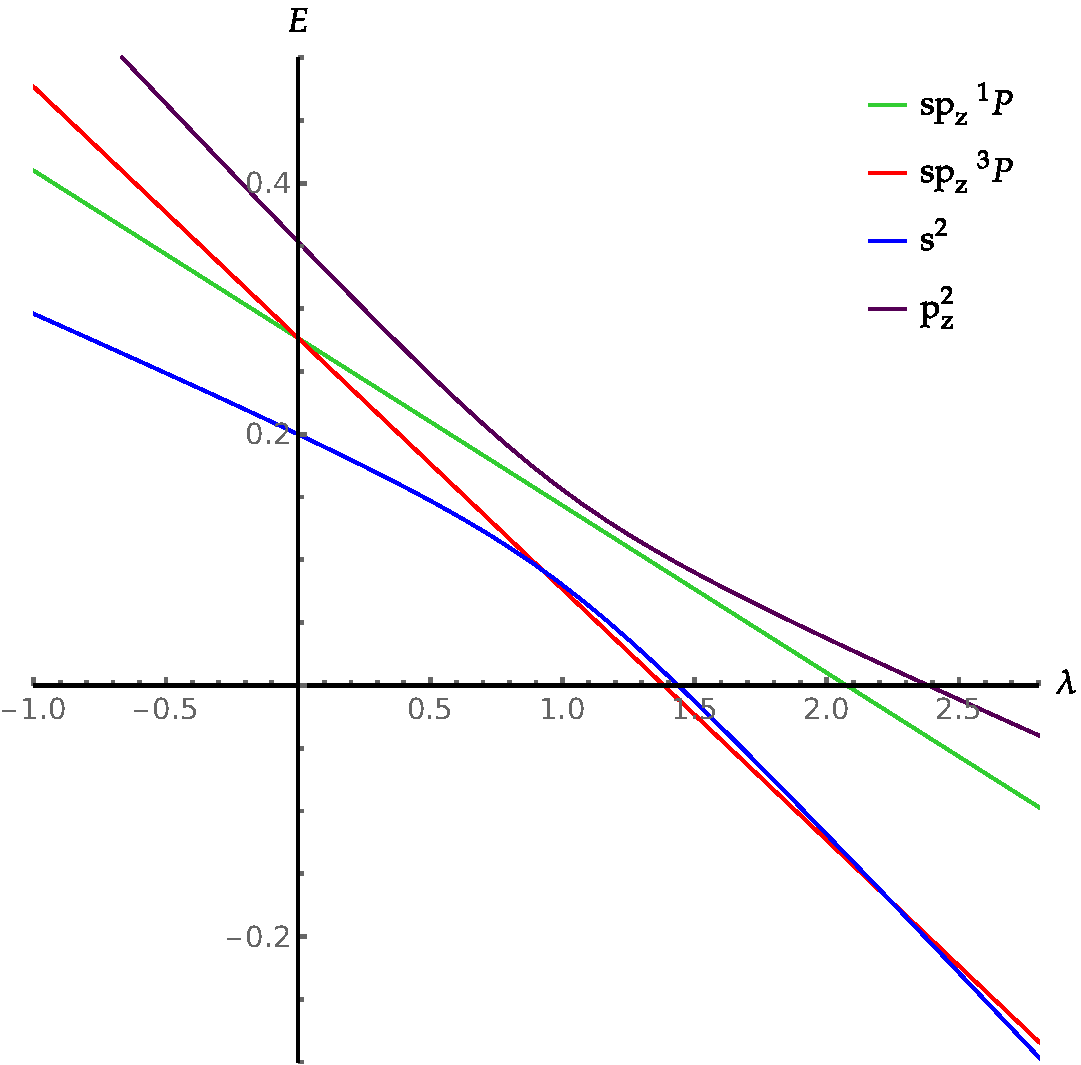
\includegraphics[width=\linewidth]{EMP_RHF_R10.pdf}
%    \caption{Energies $E(\lambda)$ in the restricted basis set \eqref{eq:rhfbasis} with $R=10$.
%    One can clearly see the avoided crossing between the $s^{2}$ and $p_{z}^{2}$ states around $\lambda = 1$.}
%    \label{fig:RHFMiniBas}
%\end{figure}
%
%To simplify the problem, it is convenient to only consider basis functions of a given symmetry. Such basis functions are called configuration state functions (CSFs). It simplifies greatly the problem because, with such a basis set, one only gets the degeneracies of interest associated with the convergence properties, \ie, the EPs between states with the same symmetry as the ground state. In the present context, the ground state is a totally symmetric singlet. According to angular momentum theory, \cite{AngularBook, SlaterBook, Loos_2009} we expand the exact wave function in the following two-electron basis:
%\begin{equation}
%\Phi_\ell(\omega)=\frac{\sqrt{2\ell+1}}{4\pi R^2}P_\ell(\cos\omega),
%\end{equation}
%where $P_\ell$ are Legendre polynomials.
%
%Then, using this basis set we can compare the different partitioning of Sec.~\ref{sec:AlterPart}. Figure \ref{fig:RadiusPartitioning} shows the evolution of the radius of convergence $R_{\text{CV}}$ as a function of $R$ for the MP, the EN, the WC and the SC partitioning in a minimal basis (\ie, consisting of $P_0$ and $P_1$) of size $K = 2$, and in the same basis augmented with $P_2$ ($K = 3$). We see that, for the SC partitioning, $R_{\text{CV}}$ increases with $R$ whereas it is decreasing for the three others partitioning. This result is expected because the MP, EN, and WC partitioning use a weakly correlated reference so $\hH^{(0)}$ is a good approximation for small $R$. On the contrary, the SC partitioning consider naturally a strongly correlated reference so the SC series converges far better when the electron are strongly correlated, \ie, when $R$ is large in the spherium model.
%
%Interestingly, the radius of convergence associated with the SC partitioning is greater than one for a greater range of radii for $K = 2$ than $K = 3$. 
%
%\begin{figure}
%    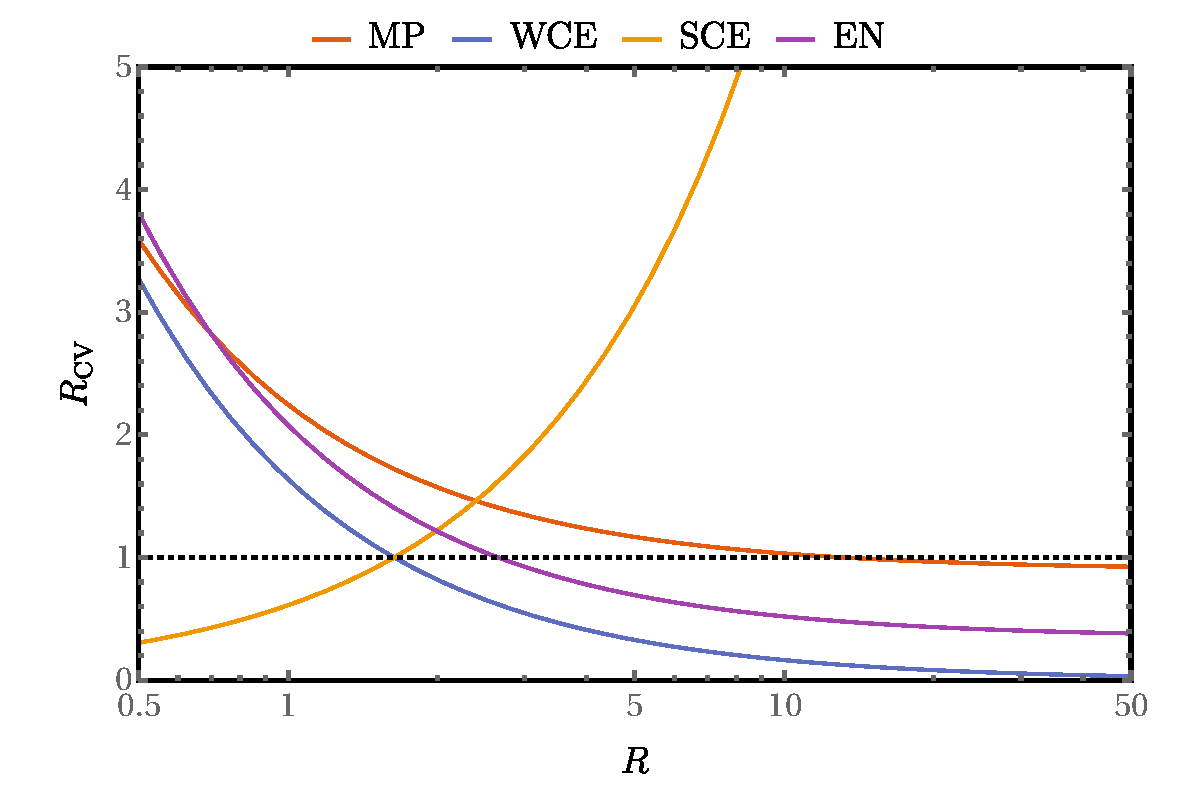
\includegraphics[width=0.49\textwidth]{PartitioningRCV2.pdf}
%    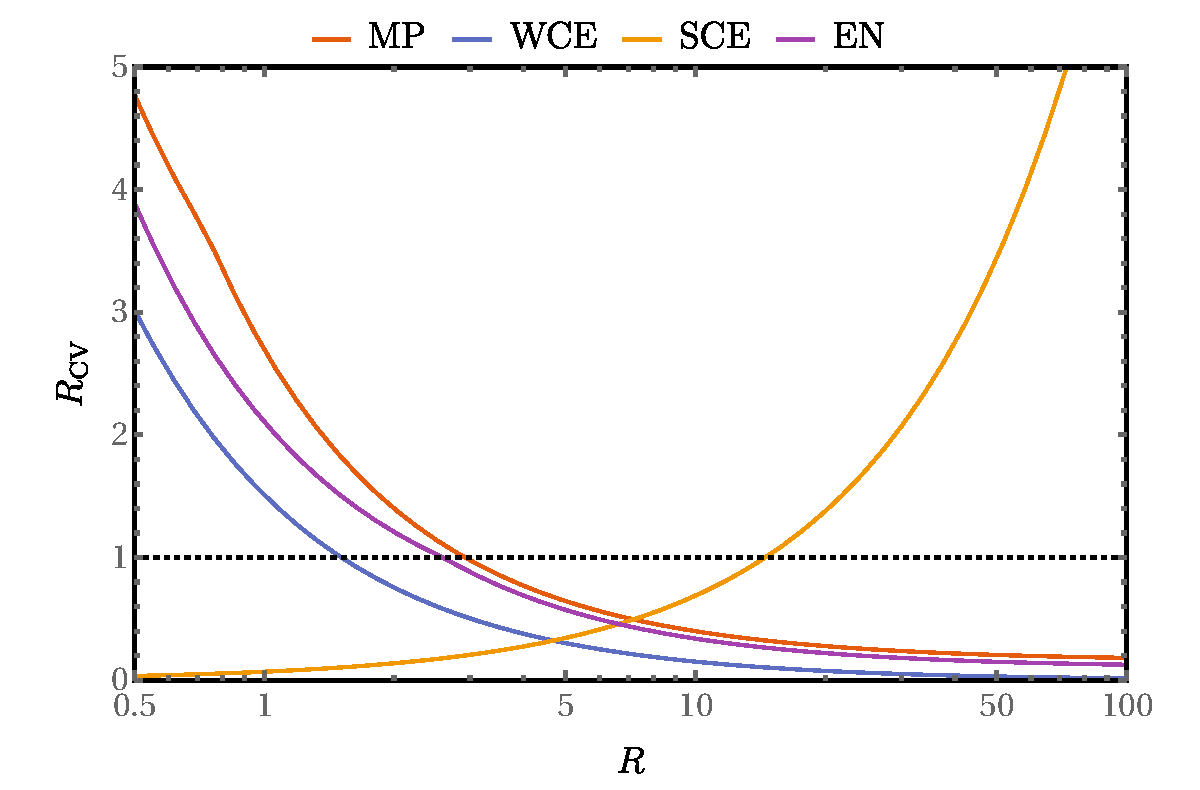
\includegraphics[width=0.49\textwidth]{PartitioningRCV3.pdf}
%    \caption{Radius of convergence $R_{\text{CV}}$ for two (left) and three (right) basis functions for various partitionings.}
%    \label{fig:RadiusPartitioning}
%\end{figure}
%
%The MP partitioning is always better than WC in Fig.~\ref{fig:RadiusPartitioning}. In the WC partitioning the powers of $R$ (the zeroth-order scales as $R^{-2}$ while the perturbation scales as $R^{-1}$) are well-separated so each term of the series has a well-defined power of $R$. This is not the case for the MP series.
%Interestingly, it can be proved that the $m$th order energy of the WC series can be obtained as a Taylor series of MP$m$ with respect to $R$. 
%It seems that the EN is better than MP for very small $R$ in the minimal basis. In fact, it is just an artefact of the minimal basis because, for $K = 3$, the MP series has a greater radius of convergence for all values of $R$. It holds true for $K>3$.
%
%
%Figure \ref{fig:RadiusBasis} shows that the radius of convergence is not very sensitive to the size of the basis set. The CSFs have all the same spin and spatial symmetries so we expect that the singularities obtained within this basis set will be $\alpha$ singularities. Table \ref{tab:SingAlpha} shows that the singularities considered in this case are indeed $\alpha$ singularities. This is consistent with the observation of Goodson and Sergeev \cite{Goodson_2004} who stated that $\alpha$ singularities are relatively insensitive to the basis set size. The discontinuities observed in Fig.~\ref{fig:RadiusBasis} for the MP partitioning are due to changes in dominant singularity. We can observe this change in Table \ref{tab:SingAlpha}, the value for $R=1$ and $R=2$ are respectively in the positive and negative planes.
%
%\begin{figure}
%    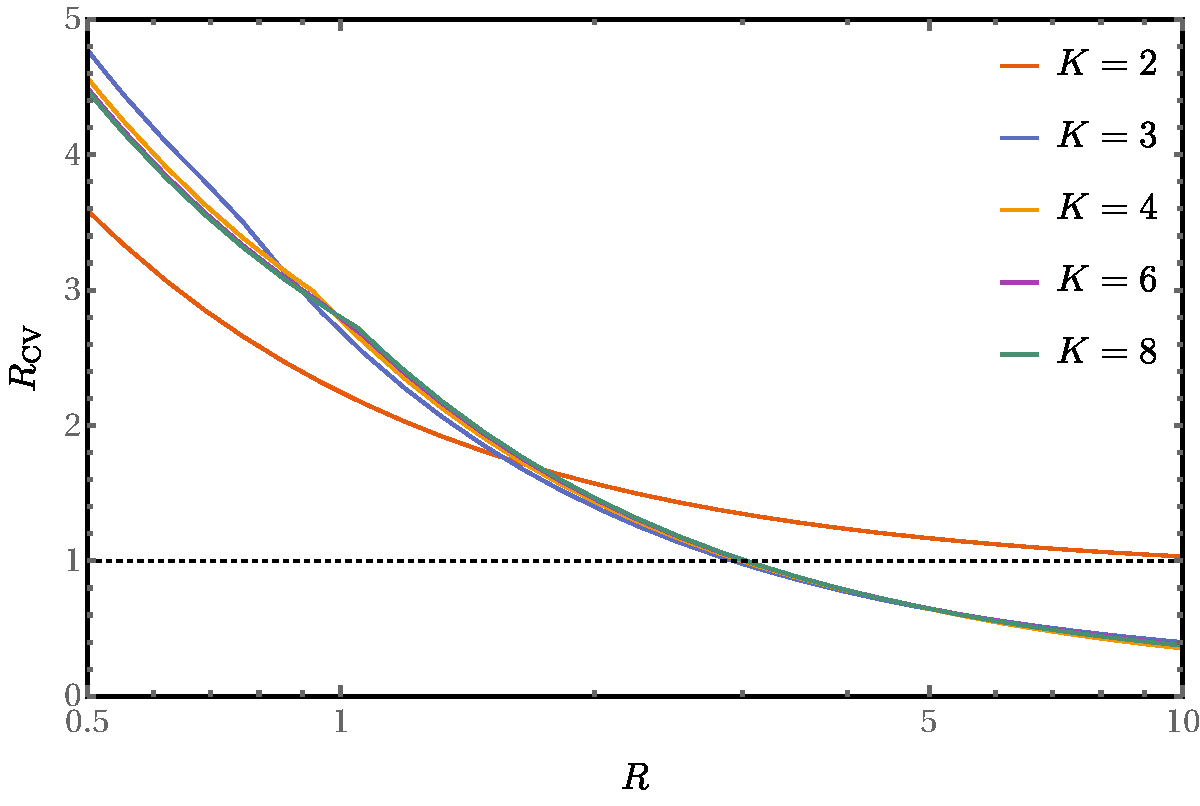
\includegraphics[width=0.49\textwidth]{MPlargebasis.pdf}
%    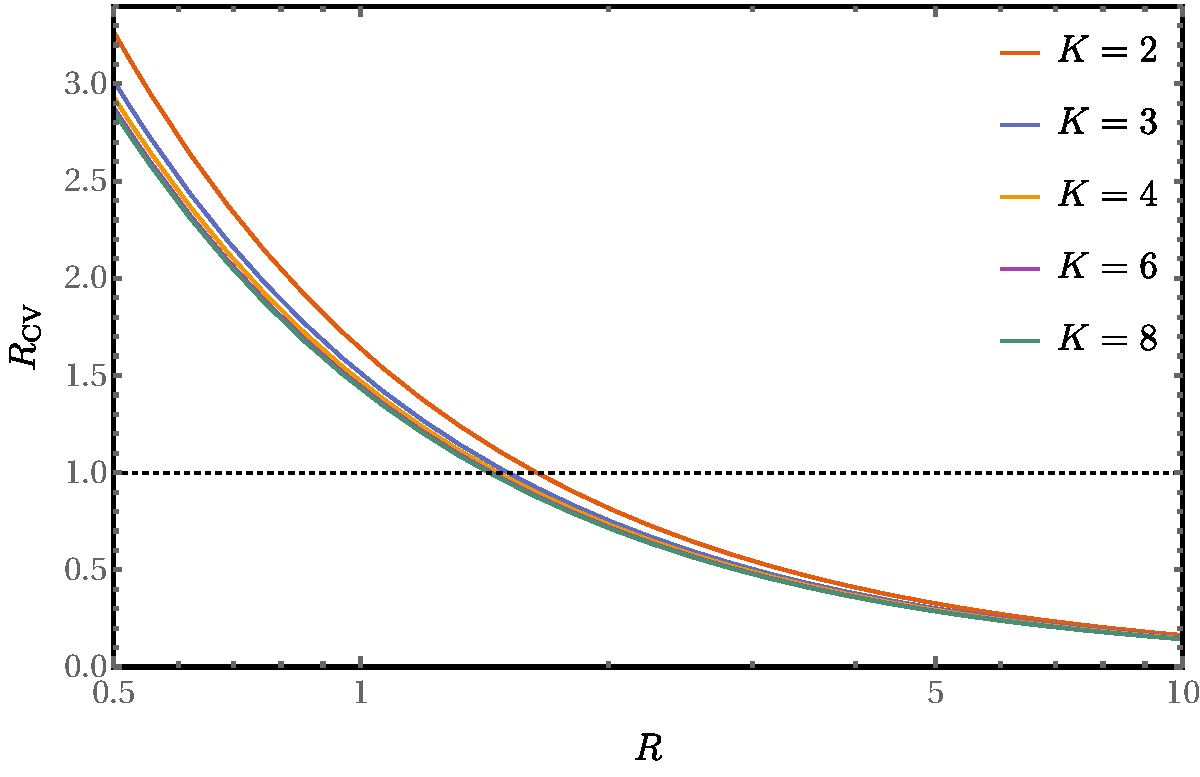
\includegraphics[width=0.49\textwidth]{WCElargebasis.pdf}
%    \caption{Radius of convergence $R_{\text{CV}}$ in the CSF basis with $K$ basis functions for the MP (left) and WC (right) partitioning.}
%    \label{fig:RadiusBasis}
%\end{figure}
%
%\begin{table*}
%\caption{Dominant singularity in the CSF basis set ($K=8$) for various value of $R$ in the MP and WC partitioning.}
%\begin{ruledtabular}
%\begin{tabular}{cccccccc}
%$R$ & 0.1 & 1 & 2 & 3 & 5 & 10 & 100 \\
%\hline
%MP & $+14.1-10.9\,i$ & $+2.38-1.47\,i$ & $-0.67-1.30\,i$ & $-0.49-0.89\,i$ & $-0.33-0.55\,i$ & $-0.22-0.31\,i$ & $+0.03-0.05\,i$ \\
%WC & $-9.6-10.7\,i$ & $-0.96-1.07\,i$ & $-0.48-0.53\,i$ & $-0.32-0.36\,i$ & $-0.19-0.21\,i$ & $-0.10-0.11\,i$ & $-0.01-0.01\,i$ \\
%\end{tabular}
%\end{ruledtabular}
%\label{tab:SingAlpha}
%\end{table*}
%
%\subsection{Exceptional points in the UHF formalism}\label{sec:uhfSing}
%
%Now, we investigate the differences in the singularity structure between the RHF and UHF formalism. To do so, we use the symmetry-broken orbitals discussed in Sec.~\ref{sec:spherium}. Thus, the UHF two-electron basis is
%\begin{align}\label{eq:uhfbasis}
% \psi_1 & =\phi_{\alpha,1}(\theta_1)\phi_{\beta,1}(\theta_2),
% & 
% \psi_2 & =\phi_{\alpha,1}(\theta_1)\phi_{\beta,2}(\theta_2),\\
% \psi_3 & =\phi_{\alpha,2}(\theta_1)\phi_{\beta,1}(\theta_2),
% & 
% \psi_4 & =\phi_{\alpha,2}(\theta_1)\phi_{\beta,2}(\theta_2).
%\end{align}
%with the symmetry-broken orbitals
%\begin{subequations}
%\begin{align}\label{eq:uhforbitals}
% 	\phi_{\alpha,1}(\theta) 
% 		& =\frac{\sqrt{75+62R}}{4\sqrt{7R}} Y_{0}(\theta)
% 		+ \frac{5\sqrt{-3+2R}}{4\sqrt{7R}} Y_{1}(\theta),
% \\ 
% 	\phi_{\beta,1}(\theta) 
%		& =\frac{\sqrt{75+62R}}{4\sqrt{7R}} Y_{0}(\theta)
%		- \frac{5\sqrt{-3+2R}}{4\sqrt{7R}} Y_{1}(\theta),
% \\
%	 \phi_{\alpha,2}(\theta) 
%	 & = - \frac{5\sqrt{-3+2R}}{4\sqrt{7R}} Y_{0}(\theta)
%	  + \frac{\sqrt{75+62R}}{4\sqrt{7R}} Y_{1}(\theta),
% \\
%	 \phi_{\beta,2}(\theta) 
%	 & =\frac{5\sqrt{-3+2R}}{4\sqrt{7R}} Y_{0}(\theta)
%	 +\frac{\sqrt{75+62R}}{4\sqrt{7R}} Y_{1}(\theta).
%\end{align}
%\end{subequations}
%
%In the UHF formalism the Hamiltonian $\hH(\lambda)$ is no more block diagonal, $\psi_4$ can interact with $\psi_2$ and $\psi_3$. The matrix elements of the Hamiltonian corresponding to this interaction are
%\begin{equation}\label{eq:MatrixElem}
%	H_{24}=H_{34}=H_{42}=H_{43}=\sqrt{R-\frac{3}{2}}\sqrt{R+\frac{75}{62}}\qty(R+\frac{25}{2})\frac{\sqrt{31}}{70R^3}
%\end{equation}
%
%For $R=3/2$ the Hamiltonian is block diagonal because the matrix elements \eqref{eq:MatrixElem} are equal to zero so this is equivalent to the RHF case but for $R>3/2$ the matrix elements become real. This interaction corresponds to the spin contamination of the wave function. For $R<3/2$ the matrix elements are complex, this corresponds to the holomorphic solution of Fig.~\ref{fig:SpheriumNrj}, the singularities in this case will be treated later. The matrix elements become real again for $R<-75/62$, this corresponds to the sb-UHF solution for negative value of $R$ observed in Sec.~\ref{sec:spherium}. We will refer to the domain where the matrix elements are complex as the holomorphic domain.
%
%The singularity structure in this case is more complex because of the spin contamination of the wave function. We can not use CSFs in this case. So when one compute all the degeneracies using Eqs.~\eqref{eq:PolChar} and \eqref{eq:DPolChar} some correspond to EPs and some correspond to conical intersections. The numerical distinction of those singularities is very difficult. We will first look at the energies $E(\lambda)$ obtained with this basis set to attribute a physical signification to the singularities obtained numerically.
%Figure \ref{fig:UHFMiniBas} is the analog of Fig.~\ref{fig:RHFMiniBas} in the UHF formalism. We see that in this case the $sp_{z}$ triplet interacts with the $s^{2}$ and the $p_{z}^{2}$ singlets. Those avoided crossings are due to the spin contamination of the wave function.
%
%\begin{figure}
%    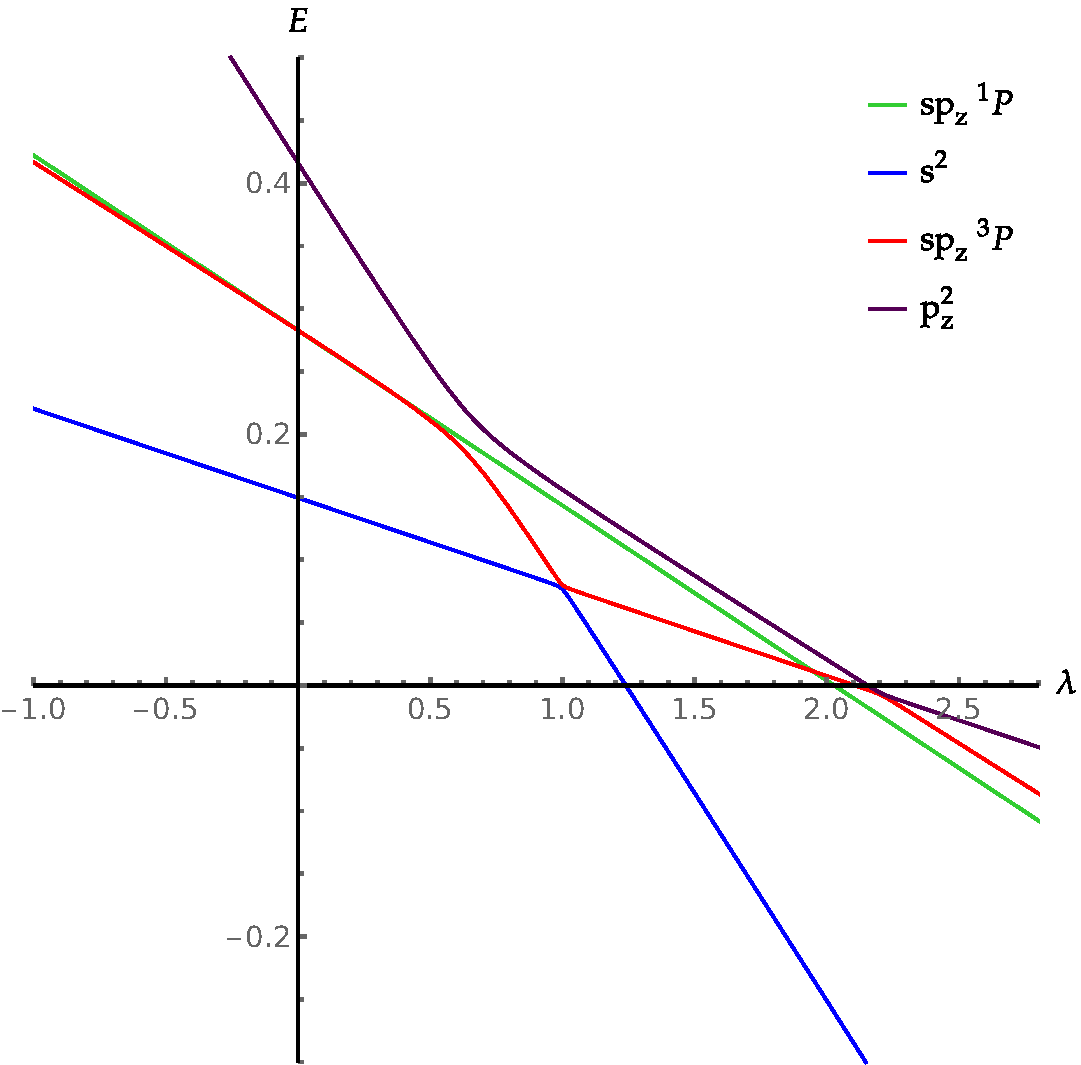
\includegraphics[width=\linewidth]{EMP_UHF_R10.pdf}
%    \caption{Energies $E(\lambda)$ in the unrestricted basis set \eqref{eq:uhfbasis} with $R=10$.}
%    \label{fig:UHFMiniBas}
%\end{figure}
%
%Within the RHF formalism, we have observed only $\alpha$ singularities and large avoided crossings but one can see in Fig.~\ref{fig:UHFMiniBas} that in the UHF case there are sharp avoided crossings which are known to be connected to $\beta$ singularities. For example at $R=10$ the pair of singularities connected to the avoided crossing between $s^{2}$ and $sp_{z}$ $^{3}P$ is $0.999\pm0.014\,i$. And the one between $sp_{z}$ $^{3}P$ and $p_{z}^{2}$ is connected with the singularities $2.207\pm0.023\,i$. However, in spherium, the electrons cannot be ionized so those singularities cannot be the same $\beta$ singularities as the ones highlighted by Sergeev and Goodson. \cite{Sergeev_2005} We can see in Fig.~\ref{fig:UHFEP} that the $s^{2}$ singlet and the $sp_{z}$ triplet states are degenerated for $R=3/2$. For $R>3/2$, it becomes an avoided crossing on the real axis and the degeneracies are $moved$ in the complex plane. The wave function is spin contaminated by $Y_1$ for $R>3/2$ this is why the $s^{2}$ singlet energy cannot cross the $sp_{z}$ triplet curves anymore. When $R$ increases this avoided crossing becomes sharper. As presented before $\beta$ singularities are linked to quantum phase transition so it seems that this singularity is linked to the spin symmetry breaking of the UHF wave function. The fact that a similar pair of $\beta$ singularities appears for $R<-75/62$ confirms this assumption. The sharp avoided crossing between $sp_{z}$ $^{3}P$ and $p_{z}^{2}$ is not present on Fig. \ref{fig:UHFEP}. The second pair of $\beta$ singularities resulting from this avoided crossing appears for $R\gtrsim 2.5$, this is probably due to an excited-state quantum phase transition but this still need to be investigated. 
%
%\begin{figure}
%    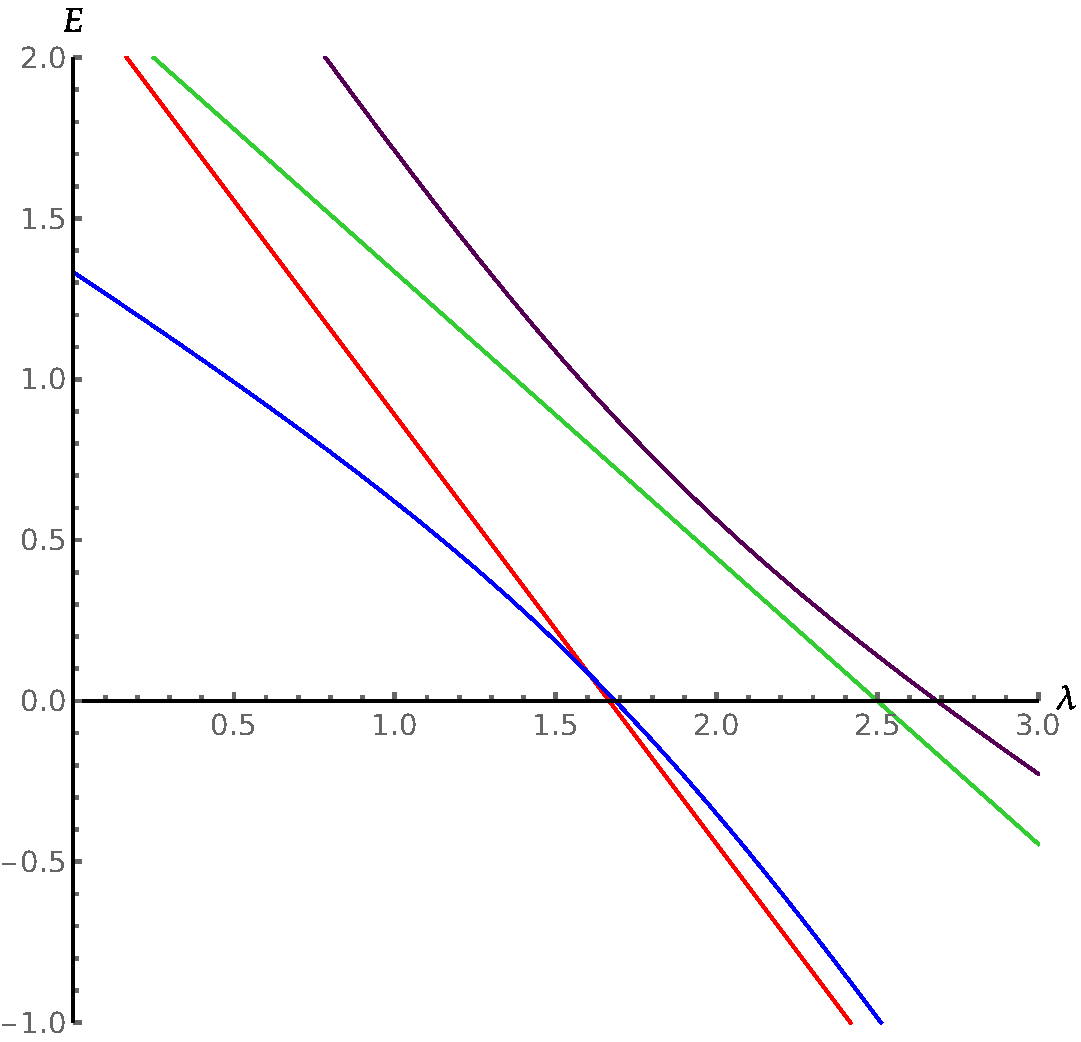
\includegraphics[width=0.45\textwidth]{UHFCI.pdf}
%    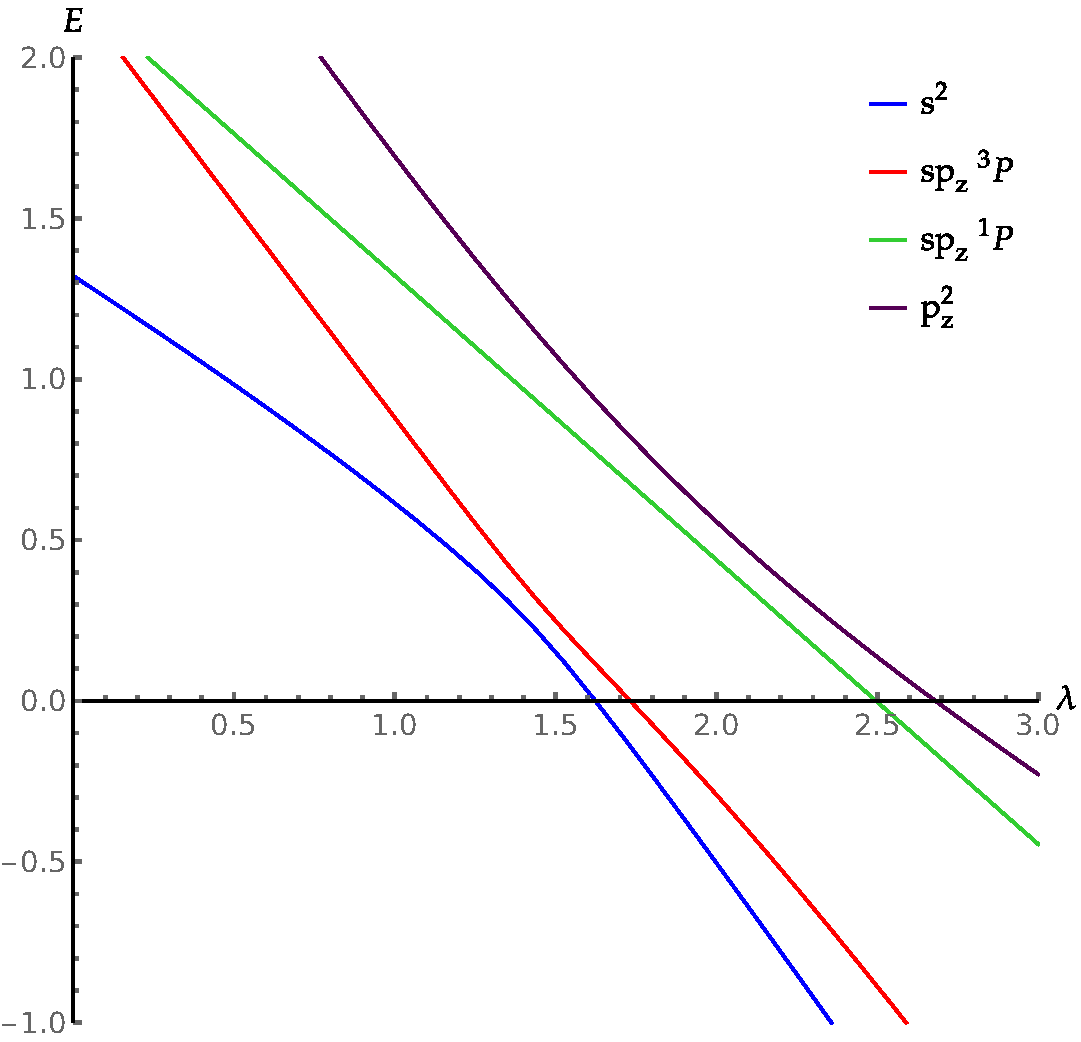
\includegraphics[width=0.45\textwidth]{UHFEP.pdf}
%    \caption{Energies $E(\lambda)$ in the unrestricted basis set \eqref{eq:uhfbasis} for $R=1.5$ (left) and $R=1.51$ (right).}
%    \label{fig:UHFEP}
%\end{figure}
%
%As shown before, some matrix elements of the Hamiltonian become complex in the holomorphic domain. Therefore the Hamiltonian becomes non-Hermitian for these values of $R$. In Ref.~\onlinecite{Burton_2019a}, Burton \textit{et al.}~proved that for the \ce{H_2} molecule the unrestricted Hamiltonian is not \pt -symmetric in the holomorphic domain. An analog reasoning can be done with the spherium model to prove the same result. The \pt -symmetry (invariance with respect to combined space reflection $\mathcal{P}$ and time reversal $\mathcal{T}$) is a property which ensures that a non-Hermitian Hamiltonian has a real energy spectrum. \cite{BenderPTBook} Thus \pt -symmetric Hamiltonians can be seen as an intermediate class between Hermitian and non-Hermitian Hamiltonians.
%
%Figure \ref{fig:UHFPT} shows that for the spherium model a part of the energy spectrum becomes complex when $R$ is in the holomorphic domain. The domain of values where the energy becomes complex is called the broken \pt-symmetry region. This is consistent with the fact that in the holomorphic domain the Hamiltonian is no more \pt -symmetric. 
%
%For a non-Hermitian Hamiltonian the EPs can lie on the real axis. In particular, at the point of {\pt} transition (the point where the energies become complex) the two energies are degenerate resulting in such an EP on the real axis. This degeneracy can be seen in Fig.~\ref{fig:UHFPT}.
%
%\begin{figure}[h!]
%    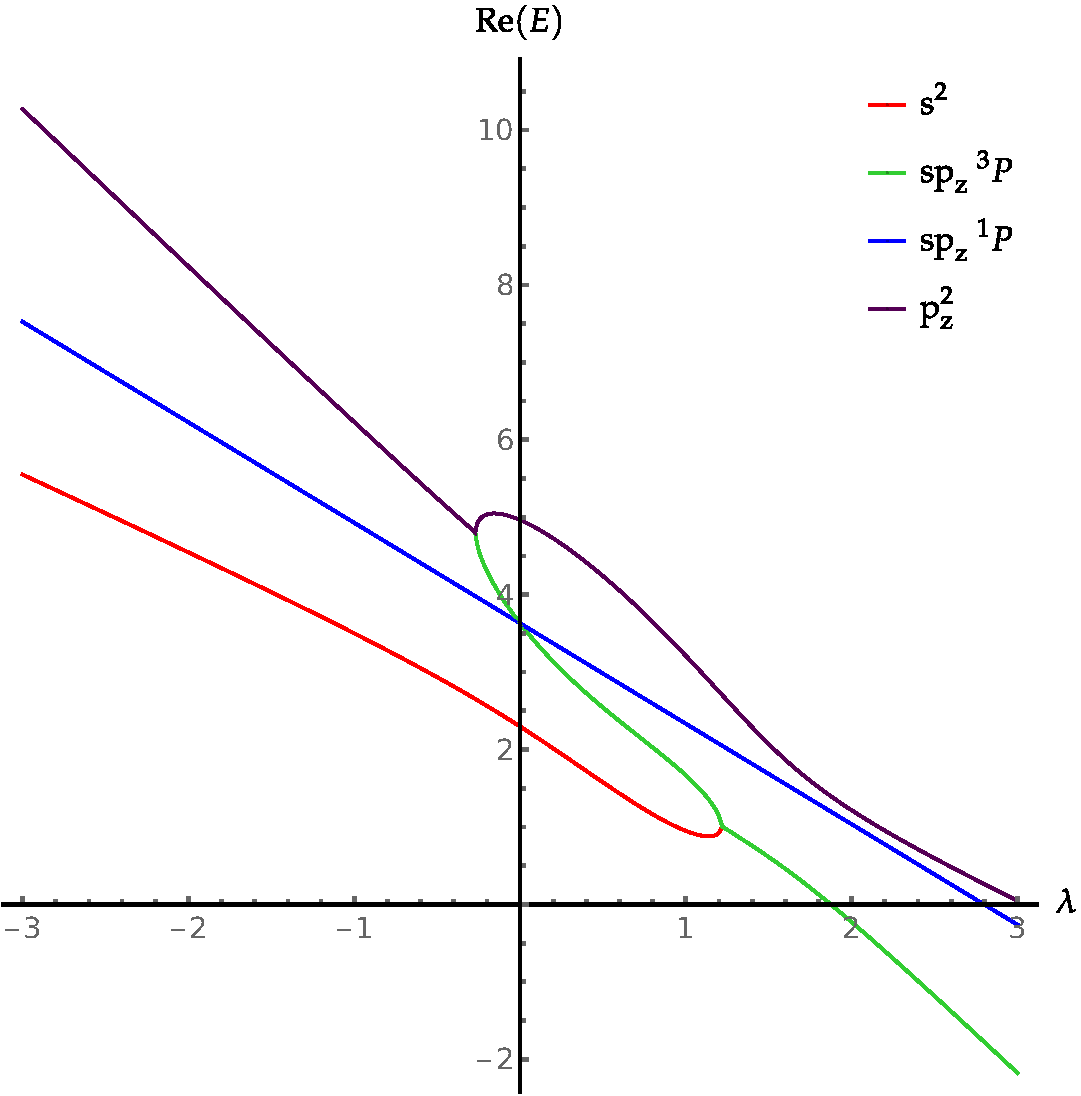
\includegraphics[width=0.45\textwidth]{ReNRJPT.pdf}
%    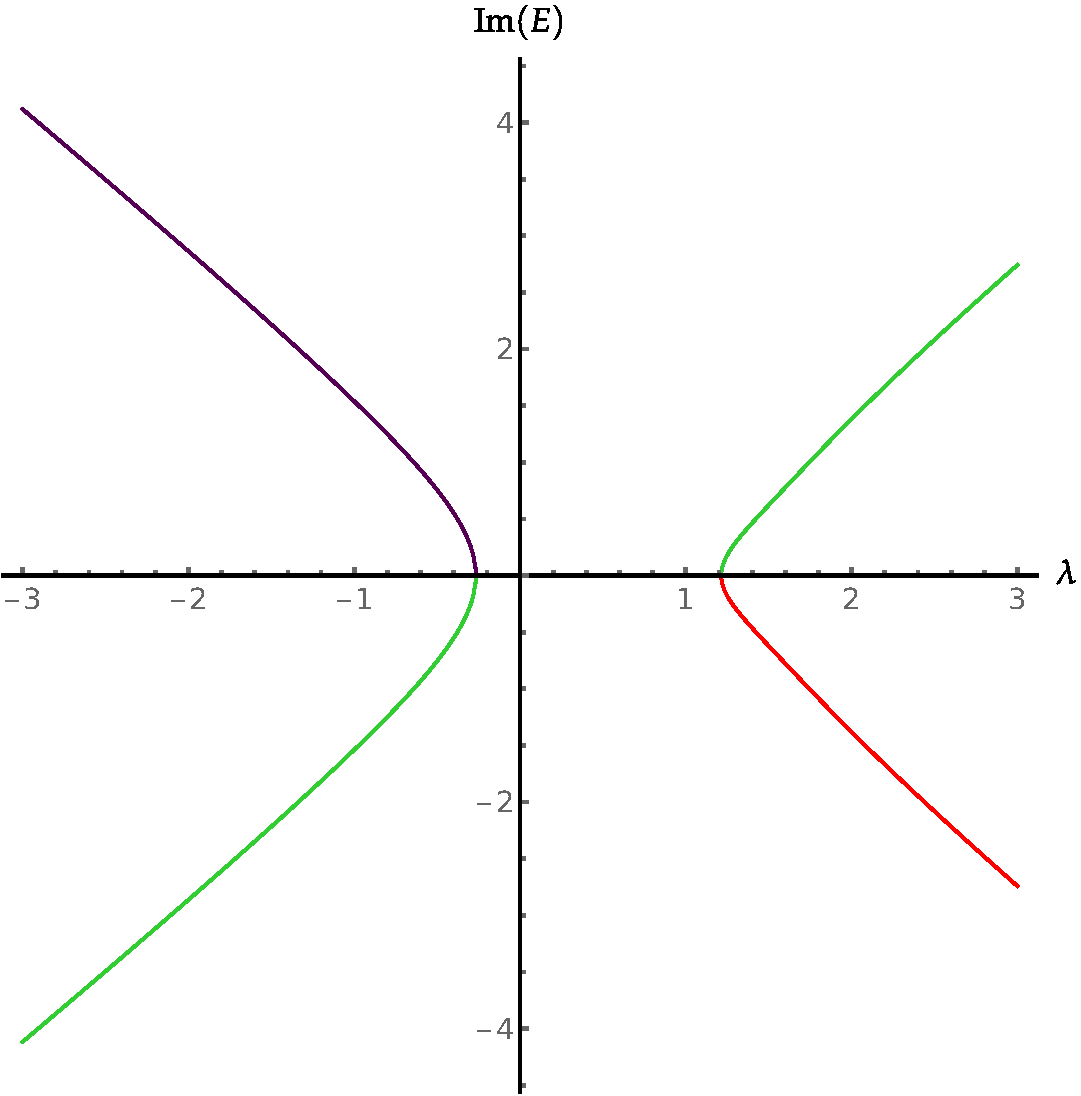
\includegraphics[width=0.45\textwidth]{ImNRJPT.pdf}
%    \caption{Real part (left) and imaginary part (right) of $E(\lambda)$ in the unrestricted basis set \eqref{eq:uhfbasis} for $R=1$.}
%    \label{fig:UHFPT}
%\end{figure}

\section{Conclusion}

In order to model accurately chemical systems, one must choose, in a ever growing zoo of methods, which computational protocol is adapted to the system of interest.
This choice can be, moreover, motivated by the type of properties that one is interested in.
That means that one must understand the strengths and weaknesses of each method, \ie, why one method might fail in some cases and work beautifully in others. 
We have seen that for methods relying on perturbation theory, their successes and failures are directly connected to the position of EPs in the complex plane. 
Exhaustive studies have been performed on the causes of failure of MP perturbation theory. 
First, it was understood that, for chemical systems for which the HF Slater determinant is a poor approximation to the exact wave function, MP perturbation theory fails too. Such systems can be, for example, molecules where the exact ground-state wave function is dominated by more than one configuration, \ie, multi-reference systems. 
More preoccupying cases were also reported. 
For instance, it has been shown that systems considered as well-understood (\eg, \ce{Ne}) can exhibit divergent behavior when the basis set is augmented with diffuse functions. 
Later, these erratic behaviors of the perturbation series were investigated and rationalized in terms of avoided crossings and singularities in the complex plane. It was shown that the singularities can be classified in two families. 
The first family includes $\alpha$ singularities resulting from a large avoided crossing between the ground state and a low-lying doubly-excited states. 
The $\beta$ singularities, which constitutes the second family, are artifacts generated by the incompleteness of the Hilbert space, and they are directly connected to an ionization phenomenon occurring in the complete Hilbert space. 
These singularities are close to the real axis and connected with sharp avoided crossing between the ground state and a highly diffuse state. 
We have found that the $\beta$ singularities modeling the ionization phenomenon described by Sergeev and Goodson are actually part of a more general class of singularities. Indeed, those singularities close to the real axis are connected to quantum phase transition and symmetry breaking, and theoretical physics have demonstrated that the behavior of the EPs depends of the type of transitions from which the EPs result (first or higher orders, ground state or excited state transitions).

%In this work, we have shown that $\beta$ singularities are involved in the spin symmetry breaking of the UHF wave function. 
%This confirms that $\beta$ singularities can occur for other types of transition and symmetry breaking than just the formation of a bound cluster of electrons. 
%It would be interesting to investigate the difference between the different type of symmetry breaking and how it affects the singularity structure. 
%Moreover the singularity structure in the non-Hermitian case still need to be investigated. 
%In the holomorphic domain, some singularities lie on the real axis and it would also be interesting to look at the differences between the different symmetry breaking and their respective holomorphic domain. 
%Furthermore, in this study we have used spherical harmonics (or combination of spherical harmonics) as basis functions which have a delocalized nature. It would also be interesting to investigate the use of localized basis functions \cite{Seidl_2018} (for example gaussians) because these functions would be more adapted to describe the strongly correlated regime. %More generally, to investigate the effect of the type of basis on the physics of EPs.
%To conclude, this work shows that our understanding of the singularity structure of the energy is still incomplete but we hope that it opens new perspectives for the understanding of the physics of EPs in electronic structure theory.


%%%%%%%%%%%%%%%%%%%%%%%%%%%%%%%%%%%%%%%%%%%%%%%%%%%%%%%%%%%%%%
\begin{acknowledgements}
%%%%%%%%%%%%%%%%%%%%%%%%%%%%%%%%%%%%%%%%%%%%%%%%%%%%%%%%%%%%%%
This project has received funding from the European Research Council (ERC) under the European Union's Horizon 2020 research and innovation programme (Grant agreement No.~863481).
HGAB gratefully acknowledges New College, Oxford for funding through the Astor Junior Research Fellowship.
%%%%%%%%%%%%%%%%%%%%%%%%%%%%%%%%%%%%%%%%%%%%%%%%%%%%%%%%%%%%%%
\end{acknowledgements}
%%%%%%%%%%%%%%%%%%%%%%%%%%%%%%%%%%%%%%%%%%%%%%%%%%%%%%%%%%%%%%

%%%%%%%%%%%%%%%%%%%%%%%%%%%%%%%%%%%%%%%%%%%%%%%%%%%%%%%%%%%%%%
\bibliography{EPAWTFT}
%%%%%%%%%%%%%%%%%%%%%%%%%%%%%%%%%%%%%%%%%%%%%%%%%%%%%%%%%%%%%%


\end{document}
